\documentclass{scrartcl}
\usepackage[utf8]{inputenc}
\usepackage[T1]{fontenc}
\usepackage{flafter}
\usepackage{graphicx}
\usepackage{appendix}
\usepackage{amsthm}
\usepackage{amsmath}
\usepackage{mathtools} %for \smashoperator
\usepackage{amsfonts}
\graphicspath{ {./figures/} }
\usepackage[algoruled, linesnumbered, noend, noline]{algorithm2e}
\usepackage{hyperref} % For URLs
\usepackage{caption} % For subfigures
\usepackage{subcaption} % Also needed for subfigures

% Command for |x| (length-of-vector-bars).
\newcommand{\norm}[1]{\lvert #1 \rvert}
\newcommand{\doublenorm}[1]{\lvert\lvert #1 \rvert\rvert}
% Command for ceil(x) (Round up to nearest integer).
\newcommand{\ceil}[1]{\lceil #1 \rceil}
\newcommand{\floor}[1]{\lfloor #1 \rfloor}
\newtheorem{theorem}{Theorem}
\newtheorem{lemma}[theorem]{Lemma}
\newtheorem{definition}{Definition}
\usepackage{xcolor}
\usepackage{bbm}

\newcommand{\hl}[1]{{\color{red}#1}} %usage \hl{<your text here>}

\newcommand{\bigo}[1]{\mathcal{O}(#1)}
\newcommand{\nenwin}{\textsc{Nenwin }}
\newcommand{\true}{\textsc{True}}
\newcommand{\false}{\textsc{False}}
\newcommand{\M}{\mathcal{M}}
\newcommand{\N}{\mathcal{N}}
\newcommand{\B}{\mathcal{B}}
\newcommand{\sgn}[1]{\text{sgn}(#1)}
% For the references
\usepackage[block=ragged]{biblatex}
\addbibresource{references.bib}

\setlength{\parskip}{1em}
\setlength{\parindent}{0pt}

\usepackage{subfiles} % Best loaded last in the preamble

\title{Nenwin: an alternative to Neural Networks}
\author{Lulof Pirée\\\footnotesize\texttt{lulof.piree@zoho.com}\\\small{Honors Academy - Eindhoven University of Technology}\\}

\begin{document}
    \maketitle
    
    \begin{abstract}
This work describes an alternative modelling framework to neural networks, based on particle simulation.
Theory is derived for optimizing models in this framework with backpropagation. 
An implementation and exploratory empirical results of optimizing a model are presented. 
Furthermore, it is proven that the framework it is Turing-complete, 
by showing informally how the new algorithm could emulate a CPU.
Finally, proposal are made how the simulation algorithm can be improved in memory and runtime efficiency.
\end{abstract}
    
    \section{Introduction}
    Neural networks, such as Multilayer Perceptrons, Recurrent Neural Networks (e.g. the GRU \cite{gru_original}),
Convolutional Neural Networks (e.g. the famous AlexNet \cite{alexnet}) and many more, 
are a popular class of trainable models for Artificial-Intelligence and datamining applications. 
Neural networks are a series of interconnected functions consisting of an affine map followed by a nonlinear activation function, 
such as the hyperbolic tangent. 
In essence, they are a trainable nonlinear functions. 
One may object that Recurrent Neural Networks are no functions, as they have a state. 
But they can be seen as a function that takes it own output back as an additional argument: 
their computation remains the same.

Simulation of physical particles is a well-established technology for scientific research, 
for example used in astronomy and chemistry. 
These simulations consist of a model incorporating physical laws, 
and individual particles that interact according to these lays.
This can for example be used to predict the motion of particles.
Many textbooks and even more articles are available on this topic, for example \cite{computer_sim_liquids}, \cite{heinz_pairlist_alg} and \cite{BEEMAN1976}.  

Humans, however, are not regarded as functions (the behavioural approach of psychology, 
which studied humans and other animals as functions, 
has now mostly been deprecated \cite{matlin2016cognition}). 
Their behaviour can change over time. 
Given the exact same environment at a later moment in time, 
humans may behave differently than they did the previous time.

This work explores a new machine learning framework based on particle simulation, 
that is designed to capture this flexibility of behaviour better. 
It is based on classical Newtonian mechanics,
so the interaction between particles can be compared to interactions between stars, planets and asteroids. 
A set of particles forms a model, and their \textit{initial} positions, 
\textit{initial} velocities and masses are their learnable parameters. 
Input data is represented by particles as well, 
and their movement is governed by gravitational interactions with the particles in the model. 
The eventual position of the input particles is used to determine the output. 
Because these input particles can also attract the particles of the model, 
the model can change its shape, which in turn changes its computations. 
Hence the algorithm encoded in the model can, 
in theory, change over time, without retraining. 

It should be noted that the new framework, to be called \textsc{Nenwin} from now onward, 
is designed for applications in which it either needs to act as an active agent, 
such as robotics or games, 
or needs to generate different output over time, 
such as music generation. 
For tasks such as image classification it does not provide any benefit over Neural Networks, 
and such tasks are only of interest for verification purposes.

All source code written for this project is available at \url{https://github.com/Nifrec/nenwin} under the open-source AGPL-3.0 licence\cite{AGPL_3}.

\subsection{Outline}
This report will begin with a description the \nenwin framework: 
the different particles involved, their parameters and the simulation algorithm. 
Also the motivation for including certain particles will be explained.

The second part of this work will elaborate on theoretical capabilities of \nenwin, namely Turing-completeness.
It will be proven, relatively informally, that \nenwin is able to simulate a CPU of the RAM model of computation,
which is equivalent in computational power to a Turing Machine.

The third section will describe how the backpropagation algorithm can be applied to a \nenwin simulation.
It will explain how various parameters are computationally related to the output of a \nenwin model,
and a loss function for a classification tasks will be defined.

The fourth section will present the empirical results of an implementation of the backpropagation algorithm.
No robust statistical analysis of the impact of hyperparameters on the performance will be given,
but instead the behaviour of the training algorithm will be elaborated for a particularly interesting run,
in learning curves and an evaluation of the changes made to the model.

The fifth and sixth section will analyse the runtime and memory issues of the implementation, 
and propose modifications for the algorithm to improve on this.
The implementation and empirical evaluation of those modifications were
unfortunately beyond the scope of this study.

Finally, the report will finish with a discussion of limitations and directions of future work,
and summarize the main points in a conclusion.



    
    \section{Algorithm Description}
    This section will describe the basic design of the \nenwin scheme. Note that \nenwin represents a class of algorithms, similar to neural networks: each network encodes a different algorithm, but the underlying mechanics are the same. Here the underlying mechanics of \nenwin will be explained.

\subsection{Objects}
\nenwin is best described by defining a family of objects known as particles. The scheme uses a subspace of $\mathbb{R}^n$, often $n=2$ is used in this report to support visualizations, but any higher dimensionality can be used as well. Each particle has a position, a velocity and an acceleration, which are all vectors in $\mathbb{R}^n$. Each particle has a mass (i.e. a decimal value, \textit{allowed to be negative}) as well, and its acceleration is at any point in governed by Newton's Second Law \cite{principia} and a force vector $\vec{f}$:
\begin{equation}
    p.acc = \frac{1}{p.mass} \sum_{\vec{f} \text{ acting on } p}\vec{f}
\end{equation}
Where $p.acc$ and $p.mass$ are the acceleration and mass of any particle $p$.

Note that these forces can only be caused by other particles. Each particle has an associated \textit{attraction function}, that describes what force the particle exerts on any other particle. Although many different functions can be used for this purpose, a natural first choice would be the gravity function (with the constant factor $G$ (the gravitational acceleration) replaced by 1):
\begin{equation}
    \norm{\vec{f}} = \frac{p_1.mass \cdot p_2.mass}{\norm{p_1.pos - p_2.pos}^2}. \label{eq:newton_grav_force}
\end{equation}
The direction of the force is the direction from the first particle to the second particle, so the force vector is given by:
\begin{equation}
    \vec{f} = \frac{p_1.pos - p_2.pos}{\norm{p_1.pos - p_2.pos}} \cdot\frac{p_1.mass \cdot p_2.mass}{\norm{p_1.pos - p_2.pos}^2}. \label{eq:newton_grav_force}
\end{equation}

Particles are divided into two general subclasses: Nodes and Marbles. Nodes are used to represent an architecture, they are the fixed part of a \nenwin network that encodes an algorithm. Nodes are further subdivided into MarbleEaterNodes and MarbleEmitterNodes, as described later. Marbles represent input and output data, and are created at runtime. Marbles can keep an optional reference to the datum they represent.

Particles \textit{experience} forces exerted on them by other particles, but also \textit{exert forces onto} other particles. Unlike in classical mechanics, \nenwin does not require these forces to be symmetric. 
To regulate the \textit{experienced} forces, each particle $p$ has the attributes \texttt{marble\_stiffness} and \texttt{node\_stiffness}. These act as multipliers for experienced forces, and are required to be real values in $[0, 1]$.
The forces that each particle $p$ exerts onto other particles, is regulated in a similar way: $p$ has two attributes\texttt{marble\_attraction} and \texttt{node\_attraction}, act as multipliers of the force that $p$ exerts onto other particles. Also these attributes must be real values in $[0, 1]$. 

To summarize, the motion of a particle $p$ is described by the following differential equations:
\begin{align}
    &p.pos = p.pos_0 + \nabla p.pos \cdot t  = p.pos_0 + p.vel \cdot t \label{eq:def_pos} \\
    &p.vel = p.vel_0 + \nabla p.vel \cdot t = p.vel_0 + p.acc \cdot t \label{eq:def_vel}\\
    &\vec{f}_{net}  = \texttt{marble\_stiffness} \cdot \sum_{\text{Mables $m$ acting on $p$}} \frac{p.mass \cdot m.mass}{\norm{p.pos - m.pos}^2} \nonumber \\
    & \qquad + \texttt{node\_stiffness} \cdot \sum_{\text{Nodes $n$ acting on $p$}} \frac{p.mass \cdot n.mass}{\norm{p.pos - n.pos}^2} \label{eq:def_f_net}\\
    &p.acc = \frac{\vec{f}_{net}}{p.mass} \label{eq:def_acc}
\end{align}
Where $t$ denotes the amount of time passed, and $p.pos_0$ and $p.vel_0$ the initial position and velocity respectively of the particle when it was created.
The acceleration of $p$ depends the forces $p$ experiences. These forces are a function of $p$'s relative distances to other Marbles and Nodes (the denominators in \eqref{eq:def_f_net} are distance measures). These distances depend on the value of $p.pos$ and the motion of other particles. Hence $p.pos$, $p.val$ and $p.acc$ are highly dependent on the other particles in a \textsc{Nenwin} model, and can change significantly even when only an very small amount of time passes.

To enable output production, a special subclass of Node called the MarbleEaterNode is used: this class stores an additional real-valued radius. When, in the simulation, the distance between a Marble and a MarbleEaterNode becomes smaller than the radius of the MarbleEaterNode, then the Marble will be removed from the simulation: it was 'eaten' by the MarbleEaterNode. The MarbleEaterNode keeps both a count of the amount of Marbles consumed, and a set of references to the associated data of the consumed Marbles.

\subsection{Motivation Emitter Nodes}
\nenwin will have a nonincreasing amount of particles if only Marbles, Nodes and MarbleEaterNode would be used.
Marbles can be removed when eaten by a MarbleEaterNode, but the there is no internal way the system can produce new Marbles (other than awaiting new input).
This would imply that the amount of information that can be stored in a \nenwin simulation is also nonincreasing in a \nenwin architecture.

Turing Machines, on the other hand, can \textit{increase} the information stored on their tape. For example, consider a Turing machine that writes down all binary numbers, starting with 0. Let this Turing machine be constructed such that it leaves a blank ('$\Box$') to the left of this 0, and then writes the next number (1), and leaves another blank and writes the next number (01), and so on. Then if given a tape of only blanks, it will continue to write an infinite amount of binary numbers on it. For any reasonable definition of information, this would clearly increase the total amount of information on the tape. 

\subsection{EmitterNode}
To make \nenwin able to increase the amount of information, we define an additional particle called the EmitterNode (or, more specifically, a MarbleEmitterNode\footnote{Note that there is no theoretical objection against creating EmitterNodes that emit other Nodes, other than the fact that EaterNodes cannot eat each other at the same time.}). This Node will create another particle at its own position when a certain condition is met.

There are many different ways to choose the exact behaviour of MarbleEmitterNodes, but in this paper we use the following:
\begin{itemize}
    \item A MarbleEmitterNode is a special case of a MarbleEaterNode, and tracks also the cumulative mass of Marbles it has consumed in a field \texttt{stored\_mass}.
    \item The MarbleEmitterNodes can only create Marbles with predefined parameters (mass, initial velocity, etc.) \textit{near} its own position.
    \item At a fixed time interval, the MarbleEmitterNode will create a new Marble and subtract its mass from \texttt{stored\_mass}, unless \texttt{stored\_mass} is smaller than the mass of the would-be created Marble. \\
    In case the mass of the Marble is negative, it will only be created as long as the \texttt{stored\_mass} is \textit{at most} the value of the mass of the Marble (i.e. the \texttt{stored\_mass} is also negative, and has a magnitude at least as great as the magnitude of the mass of the Marble).
    \item The created Marble must be within the radius or at an infinitesimal distance from the border of the radius of the MarbleEmitterNode. In case the Marble is within the radius it will be consumed immediately, hence only the infinitesimal distance is a practical option. In implementation, where infinitesimal numbers cannot be represented, a small constant $\epsilon > 0$ can be defined such that we require (if $emitter$ is the MarbleEmitterNode that creates Marble $m$):
    \begin{align}
        emitter.radius < distance(emitter.pos, m.pos) \leq emitter.radius + \epsilon
    \end{align}
	(More informally, MarbleEmitterNodes may only emit Marbles as close to the circumference of their radius as possible, but without immediately eating the Marble again).
\end{itemize}

To see how EmitterNodes can be used to create any arbitrary amount of entropy, consider an EmitterNode that generates Marbles with infinitesimally small mass, or even 0 mass. After eating a Marble with a finite mass, it will be able to generate infinitely many new Marbles. If a dynamic system guides the movement of the Marbles, then each can eventually take on a unique position (since they are not created at the same moment, and the system is dynamic, they will follow a different path). Any information can be encoded in the distribution of these Marbles, which implies that the amount of information in the simulation can be increased in the same way as a Turing Machine can increase the information on its tape.

See \ref{fig:particles_class_diagram} for a diagram the complete particle hierarchy. 

\begin{figure}[h]
    \centering
    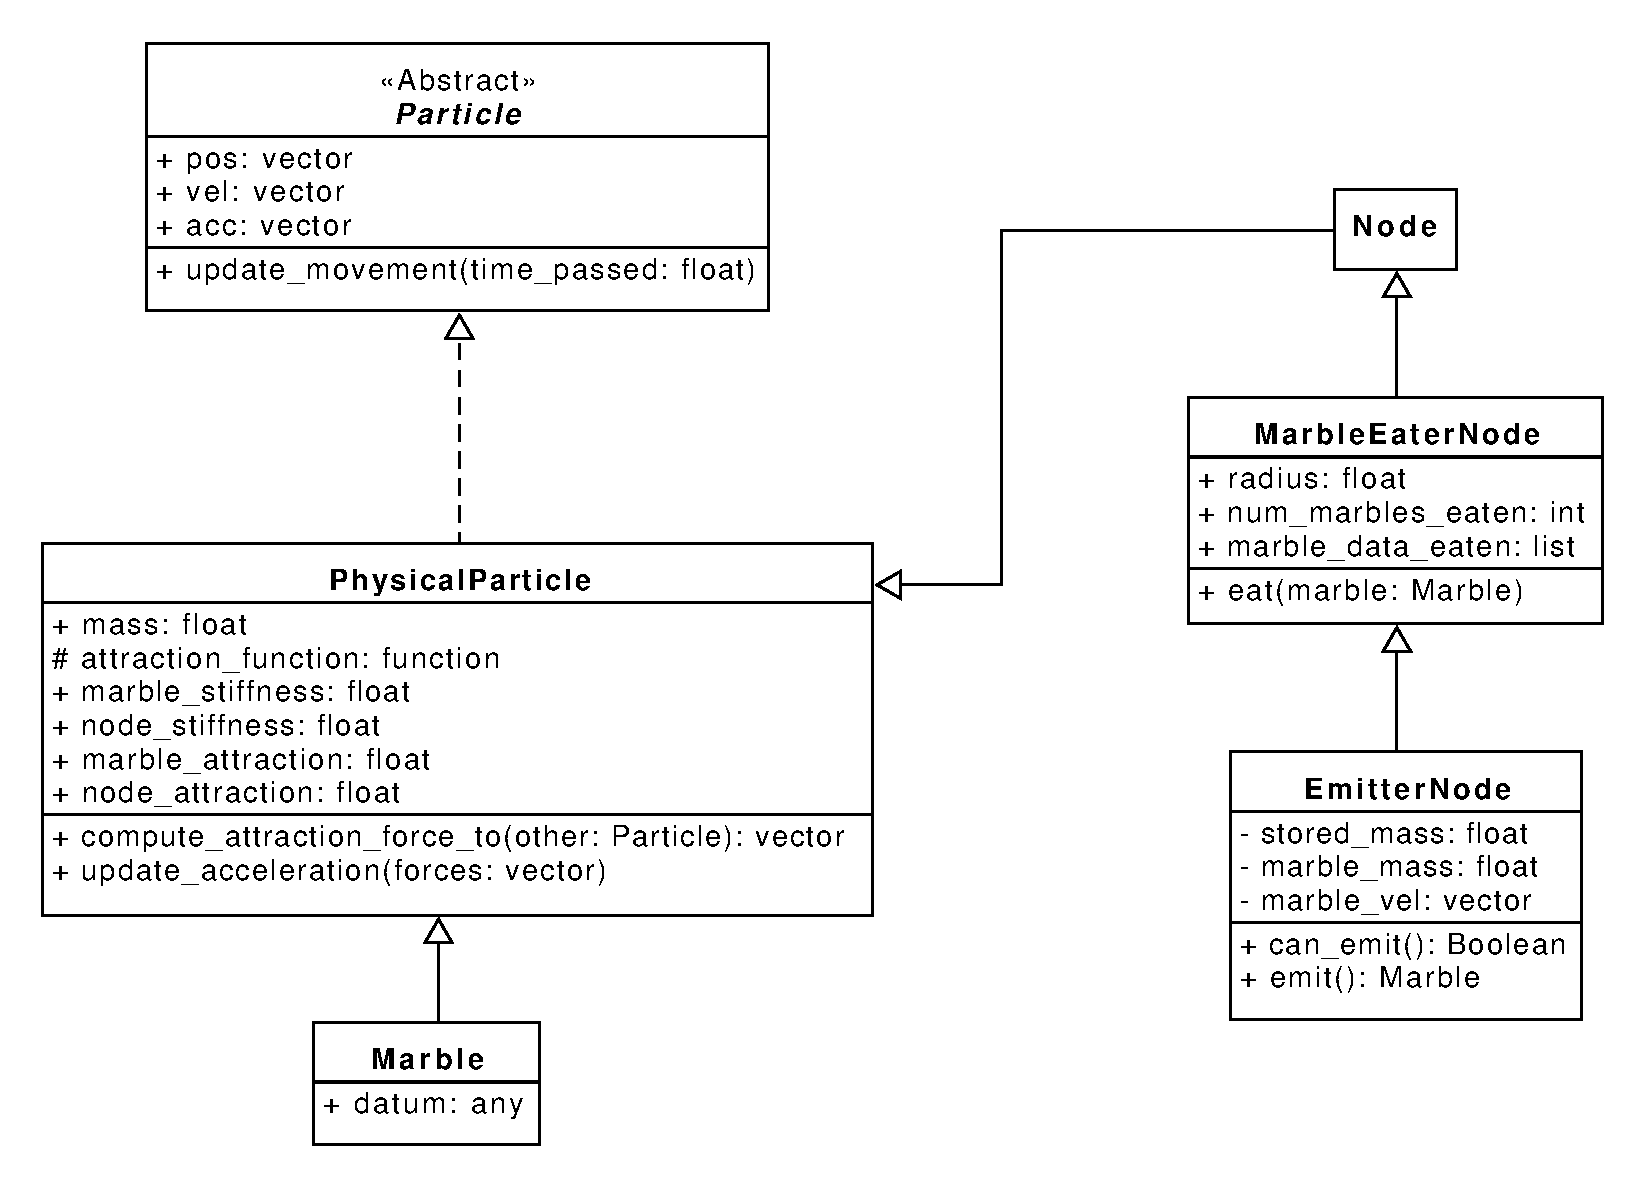
\includegraphics[scale=0.5]{figures/particles_class_diagram.pdf}
    \caption{UML class diagram depicting the inheritance relations between different particles. Note that the exact inheritance and attribute-visibilities may vary between implementations. For example, in the provided implementation, Marble is a subclass of Node.}
    \label{fig:particles_class_diagram}
\end{figure}

\subsection{Particle attributes}
An overview of the different attributes per particle subclass is given in Table \ref{table:attributes}.

\begin{table}[h]
\begin{tabular}{llllll}
\textbf{Attribute} & \textbf{type} & \textbf{Marble} & \textbf{Node} & \textbf{MarbleEaterNode} & \textbf{EmitterNode} \\ \hline
\multicolumn{1}{l|}{\texttt{pos}}                  & \multicolumn{1}{l|}{$\mathbb{R}^n$} & \checkmark & \checkmark & \checkmark & \checkmark \\
\multicolumn{1}{l|}{\texttt{vel}}                  & \multicolumn{1}{l|}{$\mathbb{R}^n$}               & \checkmark & \checkmark & \checkmark & \checkmark \\
\multicolumn{1}{l|}{\texttt{acc}}                  & \multicolumn{1}{l|}{$\mathbb{R}^n$}               & \checkmark & \checkmark & \checkmark & \checkmark \\
\multicolumn{1}{l|}{\texttt{marble\_stiffness}}    & \multicolumn{1}{l|}{{[}0, 1{]}}     & \checkmark & \checkmark & \checkmark & \checkmark \\
\multicolumn{1}{l|}{\texttt{node\_stiffness}}      & \multicolumn{1}{l|}{{[}0, 1{]}}     & \checkmark & \checkmark & \checkmark & \checkmark \\
\multicolumn{1}{l|}{\texttt{marble\_attraction}}   & \multicolumn{1}{l|}{{[}0, 1{]}}     & \checkmark & \checkmark & \checkmark & \checkmark \\
\multicolumn{1}{l|}{\texttt{node\_attraction}}     & \multicolumn{1}{l|}{{[}0, 1{]}}     & \checkmark & \checkmark & \checkmark & \checkmark \\
\multicolumn{1}{l|}{\texttt{attraction\_function}} & \multicolumn{1}{l|}{$f:\mathcal{P}\times\mathcal{P}\rightarrow \mathbb{R}^n$}       & \checkmark & \checkmark & \checkmark & \checkmark \\
\multicolumn{1}{l|}{\texttt{datum}}                & \multicolumn{1}{l|}{any object}     & \checkmark &   &   &   \\
\multicolumn{1}{l|}{\texttt{eaten\_marbles}}       & \multicolumn{1}{l|}{stack of Marbles} &   &   & \checkmark & \checkmark \\
\multicolumn{1}{l|}{\texttt{radius}}               & \multicolumn{1}{l|}{$\mathbb{R}$}           &   &   & \checkmark & \checkmark \\
\multicolumn{1}{l|}{\texttt{stored\_mass}}       & \multicolumn{1}{l|}{$\mathbb{R}$} &   &   & \checkmark & \checkmark \\
\multicolumn{1}{l|}{\texttt{spawnpos}}             & \multicolumn{1}{l|}{$\mathbb{R}^n$}            &   &   &   & \checkmark \\
\multicolumn{1}{l|}{\texttt{prototype\_marble}}    & \multicolumn{1}{l|}{Marble}         &   &   &   & \checkmark
\end{tabular}
\caption{A summary of different attributes used by different particles. $\mathcal{P}$ is used to denote the set of all particles in a given architecture. \newline
Here \texttt{pos}, \texttt{vel} and \texttt{acc} are the position, velocity and acceleration of a particle, which are real vectors defined in $\mathbb{R}^n$ where $n$ is the dimensionality of the architecture. The stiffness and attraction values are real numbers in the interval $[0, 1]$. The attraction function maps two particles to a vector of the same shape as \texttt{acc}.\newline
The \texttt{datum} is any data-element that a Marble represents, and this attribute is allowed to be valueless.\newline
\texttt{eaten\_marbles} is a stack of all Marbles a MarbleEaterNode (or its subclass, a MarbleEmitterNode) has consumed, with the latest consumed Marble on top of the stack. This stack is allowed to be empty. \newline
The \texttt{radius} of a MarbleEaterNode is the maximum distance such that, if a Marble is at this distance or at a smaller distance to the MarbleEaterNode, it will be consumed. \\
The \texttt{stored\_mass} is the cumulative mass of the Marbles in \texttt{eaten\_marbles} of a MarbleEmitterNode, minus the cumulative mass of emitted Marbles. This value is allowed to be negative, which is required to emit negatively-massed Marbles. \newline
The \texttt{spawnpos} is the relative position from the center of an MarbleEmitterNode at which a Marble can be created when emitted, this point is at most \texttt{radius} + $\epsilon$ away from the center of the MarbleEmitterNode, where $\epsilon$ is an infinitesimal number. The prototype Marble is a 'blueprint' of the Marble that is emitted: all its attributes are copied to a new Marble that is being emitted, except the position (which is governed by the combination of the position of the MarbleEmitterNode and \texttt{spawnpos}), the velocity and the acceleration (which are set to $\vec{0}$).}
\label{table:attributes}
\end{table}

\clearpage
\subsection{AI application}
\nenwin is designed to fulfil the role of a decision-making agent, for example as an alternative to neural networks in reinforcement learning or classification tasks. Besides the particle simulation, this would also require the system to receive input and produce output. 

For example, if a \nenwin simulation is used as an agent to play a game, say chess, then it must be able to perceive the current state of the game, and to choose a move to make. As for another example, if a \nenwin simulation is used for an image classification task, then it must be able to read the images, and output a predicted class.

Adding inputs is straightforward: a region in $\mathbb{R}^D$ (where $D$ is the chosen dimensionality of the \nenwin architecture) is chosen as the \textit{input region} $R$. If input datapoints are given in $\mathbb{R}^n$, then one can define a function (an \textit{input placer}) that maps $\mathbb{R}^n$ to a set of Marbles located in $R$. The inputs can be stored in an bi-directional input/output buffer, called a \textit{channel}. The simulation will then check the channel each timestep, and map any data in the channel to Marbles, and insert these into the simulation.

To produce output, MarbleEaterNodes are used. At each timestep, the simulation outputs a vector containing a natural number for each present MarbleEaterNode into the output of the channel. These natural numbers encode the total number of Marbles eaten by each MarbleEaterNode. This vector can, for example, be interpreted as a one-hot encoding for classification (it contains only one '1' when read as soon as the first Marble has been eaten).
For even more detailed output, one can allow external functions to read the exact set of Marbles eaten by each MarbleEaterNode. This latter extension was used for classification training described in a later section.

\subsubsection{Input Placement}
Marbles are used to represent input data, which can either be tabular data, an image, a stream of sound or video, etc.
From the algorithm's side, as described in \ref{alg:Nenwin_V1}, 
this simply means that a new set of Marbles can be added to the simulation at each timestep.
However, it is required to map the input data (together with a designated \textit{input region}) to a set of Marbles first, by means of an \textit{input placer}.
This can be done in very many ways. For example, a datapoint could be used to generate a single Marble, in which the datum is mapped to an attribute of the Marble, such as the position, the mass, the velocity, etc.. It is also possible to use information multiple datapoints to create a single Marble. Furthermore, it is also possible to define a trainable input placer, which can be optimized using marchine learning techniques.

It was chosen to use an input placer (the "GridInputPlacer") that simply spreads the Marbles evenly in a grid over the input region (in order of the input vector, from left to right, top to bottom). This input placer creates a Marble for each datapoint.
Note that this choice is rather arbitrary: as of current there are no arguments why aligning the Marbles in another pattern (such as on a circle) would be less effective.

Two variants of the GridInputPlacer were used:
\begin{itemize}
	\item MassInputPlacer: maps each datapoint to a Marble, whose mass is set to the value of the datapoint. The velocity is set to $\vec{0}$.
	\item VelInputPlacer: maps each datapoint to a Marble, whose velocity is set to a vector of which each element equals the value of the datapoint. It sets the mass of each Marble to 1.0.
\end{itemize}

All variants set, for each Marble, the remaining attributes as follows:
\begin{itemize}
	\item the radius of the threshold radius to 100.
	\item the acceleration to $\vec{0}$.
	\item the \texttt{marble\_stiffness} to 1.
	\item the \texttt{node\_stiffness} to 0.
	\item the \texttt{marble\_attraction} to 0
	\item the \texttt{node\_attraction} to 1.
\end{itemize}



\subsubsection{Simulation}
See Algorithm \ref{alg:Nenwin_V1} below for an abstract pseudocode description how a \nenwin can be simulated. This pseudocode includes input-output handling. Note that in implementation the functionality will be subdivided into different modules. 
It is for example equally fast, but from an Object-Oriented point of view preferable, to first create Marble instances for new inputs and then sending them over the channel rather than sending the raw data itself. This does not affect the behaviour of the algorithm.

\begin{algorithm}[h]
	\caption{\\\textsc{Nenwin}\textnormal{\texttt{(nodes, input\_space, placement\_function, mass\_function, channel, attraction\_function)}}}
	\label{alg:Nenwin_V1}
	\newcommand{\dataStyle}[1]{\textbf{\texttt{#1}}}
	\SetAlgoLined
	\SetKwSty{texttt}
	\SetDataSty{dataStyle}
	% Setup variables
	\SetKwData{nodes}{nodes}
	\SetKwData{input}{input\_space}
	\SetKwData{placement}{input\_placer}
	\SetKwData{channel}{channel}
	\SetKwData{node}{Node}
	\SetKwData{grav}{attraction\_function}
	\SetKwData{mass}{mass\_function}
	\SetKwData{eaters}{eater\_nodes}
	\SetKwData{emitters}{emitter\_nodes}
	% Input and output
	\KwIn{
		\nodes: A set of \node objects, each having a position, velocity and acceleration in $\mathbb{R}^D$ and a stiffness and a mass in $\mathbb{R}$.\\
		\input: A (hyperrectangular) subspace of $\mathbb{R}^D$.
		\placement: A function that maps input vectors (in $\mathbb{R}^n$) to Marbles located in \input.\\
		\channel: A bi-directional communication channel over which any finite real-valued vectors can be sent.\\
		\grav: A function that maps two Marbles (usually using their masses and their relative distance) to an attraction force vector.		
	}
	\KwOut{\texttt{None}}
	$particles \leftarrow \nodes$ \;
	$\eaters \leftarrow [node: node \in \nodes \land node \text{ is a } \textsc{MarbleEaterNode}]$ \;
	\tcc{The following is a subset of 'eaters':}
	$\emitters \leftarrow [node: node \in \nodes \land node \text{ is a } \textsc{MarbleEmitterNode}]$ \;
	\While{\texttt{True}}{
		\If{there is input on the channel}{
			\For{$\vec{v} \in \channel$}{
				$particles \leftarrow particles \cup \{\placement(\vec{v})\}$\;
			}
		}
		\If{there is an output request on the channel}{
			$output \leftarrow \text{ a new empty list}$ \;
			\For{$node \in \eaters$}{
			    $output.append(node.num\_marbles\_eaten)$ \;
			}
			Place $output$ on the channel \;
		}
		\For{$p \in particles$}{
			$\vec{f} \leftarrow \sum_{o \in particles \setminus\{p\}} \frac{o.pos - p.pos}{\doublenorm{o.pos - p.pos}} \cdot \grav(p, o)$ \;
			\tcc{Newton's Second Law}
			$p.acc \leftarrow p.mass \cdot \vec{f}$ \;
		}
		\For{$e \in \emitters$}{
		    \If{$\norm{e.stored\_mass} \geq \norm{e.prototype\_marble.mass} \land \sgn{e.stored\_mass} = \sgn{e.prototype\_marble.mass}$}{
		    $particles \leftarrow particles \cup (\text{a copy of $e.prototype\_marble$ at position $e.pos + e.spawnpos$})$
		    }
		}
		\For{$particle \in particles$}{
			Compute and update $particle$'s next position and velocity given their current acceleration (using numerical integration). \;
		}
		\For {$marble \in particles \setminus nodes$}{
			\For{$node \in \eaters$}{
				\If{$distance(marble.pos, node.pos) \leq node.radius$}{
					$particles \leftarrow particles \setminus \{marble\}$ \;
					$node.stored\_mass \leftarrow node.stored\_mass + marble.mass$ \; $node.eaten\_marbles \leftarrow node.eaten\_marble \cup \{marble\}$\;
				}
			}
		}
		}
\end{algorithm}

\clearpage    
    
    \section{Reductions}
    \textsc{Nenwin} is able to simulate other computational mechanisms \footnote{or, equivalently, other computational mechanisms can be reduced to \textsc{Nenwin}. 'Reduction' causes less ambiguity than 'simulate', as \textsc{Nenwin} is implemented via an simulation itself.}. In particular, this section will demonstrate that \textsc{Nenwin} is able to simulate all required components to implement a CPU. A CPU is an implementation of the RAM-model, which is equivalent to a Turing machine \cite{RAM_cook_reckhow}.

This section will demonstrate that \textsc{Nenwin} is able to simulate the following components, when using Marbles as data-carrying signals:
\begin{itemize}
    \item A Boolean NAND-gate with interfaces that use Marbles to transmit and receive information. Note that compositions of NAND-gates can be build to simulate all logical functions such as OR, AND, NOT, NOR, etc.
    \item A single-bit register that can store a state 0 or 1. Note that an arbitrary large composition of bit registers can store an arbitrary large amount of data.
    \item A clock that creates periodically a signal.
    \item A 'divider': a component that upon intercepting one Marble, creates multiple Marbles with velocities in different directions. In the context of wires and electricity such devices are not needed, but in the context of discrete Marbles it is required.
\end{itemize}

These reductions are not necessary of any practical use, as it is slower than directly implementing/simulating the other computational mechanisms, but it demonstrates that \textsc{Nenwin} is theoretically powerful enough to solve the same problems as these mechanisms.
These reductions use very artificial hand-made (in contrast to automatically optimized) architectures that do not use the dynamic nature of \nenwin: using immovable Nodes result in simpler proofs than with moving Nodes. 

\nenwin is by default non-terminating, but it can simulate terminating algorithms when a consistent rule is used when to read output.
One natural such rule is to read output when all Marble's have disappeared, as the output will not change anymore after this point.

Consider a variant of Newton's gravity function, called the 'threshold gravity', that rounds the force to 0 when the radius is sufficiently large:
\begin{equation}
    threshold\_gravity(p_1, p_2, \theta) = \begin{cases}
        \vec{0} & \text{ if } \norm{p_1.pos - p_2.pos} > \theta \\
        \frac{p_1.m \cdot p_2.m}{\norm{p_1.pos - p_2.pos}^2} & \text{otherwise}
        \end{cases} \label{eq:tresholdgrav}
\end{equation}

Unless stated otherwise, this threshold-gravity force function \eqref{eq:tresholdgrav} will be used as attraction function by all particles in this section.

\subsection{NAND-gate}
The \textsc{Nenwin}-scheme is able to simulate a logical NAND-gate.
As a NAND-gate is a Boolean function with only two Boolean input values, there are only 4 different input combinations that need to be handled correctly. Below it is shown how \textsc{Nenwin} can directly simulate a NAND-gate with inputs and output to the \textsc{Nenwin} program itself, and how a NAND-gate can be embedded in a larger circuit within a \textsc{Nenwin}-architecture. 

Let $\mathcal{M}$ denote the set of all possible marbles and $\mathcal{N}$ the set of all possible nodes. 
\begin{lemma}[NAND-gate]
There exists an input placer mapping a vector of two Boolean variables to a set of Marbles $f:\{0, 1\}^2 \rightarrow\mathcal{M}^2$,
a \textsc{Nenwin} architecture of only nodes $A \subseteq \N$, and a function to map the \nenwin output to a Boolean output $g:\mathbb{N}^2 \rightarrow \{\false, \true\}$,\\
such that for two Boolean variables $b_1, b_2 \in \{\false, \true\}$, $g(\vec{y}) = \neg (b_1 \land b_2)$, where $\vec{y}$ is the output harvested from architecture $A$ with input $\{f(b_1), f(b_2)\}$ after all marbles were removes from the network.
\label{lemmma:nand_simple}
\end{lemma}
\begin{proof}

    For all particles we will use \texttt{node\_stiffness} = 0, 
    \texttt{marble\_stiffness} = 1, \texttt{node\_attraction}=0 and \texttt{marble\_attraction}=1.

    Define 
    \begin{equation}
        f(b) = \begin{cases}
            &\texttt{Marble}(pos=[10, 0], vel=\vec{0}, acc=\vec{0}, mass=+10, datum=\textsc{True}) \quad \text{if $b = \textsc{True}$} \\
            &\texttt{Marble}(pos=[10, 0], vel=\vec{0}, acc=\vec{0}, mass=-10, datum=\textsc{False}) \quad \text{if $b = \textsc{False}$}
        \end{cases}
    \end{equation}
    
    Let
    \begin{align}
        A = &[ \nonumber \\
        & \texttt{MarbleEaterNode}(pos=[0, 0], vel=\vec{0}, acc=\vec{0}, mass=+10, radius=5) \nonumber \\
        & \texttt{MarbleEaterNode}(pos=[20, 0], vel=\vec{0}, acc=\vec{0}, mass=-10, radius=5) \nonumber \\
        &]
    \end{align}

    Define 
    \begin{equation}
        g(\vec{y}) = \begin{cases}
                    \false &\text{if } y[0] = 2 \\
                    \true &\text{if } y[0] \in \{0, 1\}
        \end{cases}
    \end{equation}
    
    Note that the Marbles are placed in the middle of the line-segment between the two Nodes, 
    and that positive masses attract positive masses and repel negative masses, and vice versa. 
    Hence each of the two Marbles will be accelerated in a straight line to the Node with the same polarity of mass as itself, 
    and will be eaten by it.
    
    Now if the input is $(\true, \true)$, both Marbles will have a positive mass of 10, and both will be attracted to the left Node (at $pos[0] = 0$ with mass +10). This way both will be absorbed by the first Node, and the output will read $g(\begin{bmatrix}2\\0\end{bmatrix}) = \false$ as expected.
    
    If the input equals $(\true, \false)$, $(\false, \true)$, $(\false, \false)$, then at least one Marble will be attracted and eaten by the right node (at $pos[0] = 20$ with mass -10), and since there are only 2 Marbles, no more than one Marble will be eaten by the left Node, and the output is $g(\begin{bmatrix}1\\1\end{bmatrix})$ or $g(\begin{bmatrix}0\\2\end{bmatrix})$, either of which will evaluate to $\true$ as expected.
\end{proof}
See Fig. \ref{fig:nand_simple} for a visualization of the proof.

\begin{figure}[h]
	\centering
	
\includegraphics[scale=1.5]{figures/nand_simple.pdf}
	\caption{Construction of a NAND-gate in \nenwin as used by the proof of Lemma \ref{lemmma:nand_simple}. The left Node has a positive mass, and the right Node a negative mass. Note that only one dimension (the $x$-axis) is used, and that both Marbles are placed by the input placer on exactly the same position (at $x = 10$).}
	\label{fig:nand_simple}
\end{figure}
\clearpage

The above lemma does not show how a NAND-gate can be implemented as part of a larger circuit. To achieve this, all that is needed is a NAND-gate that has a finite region of $\mathbb{R}^3$ in which it attracts particles (so that the rest of the circuit can be implemented safely outside this region), and interfaces to the other parts of the circuit. 

In this series of proofs, such interfaces are represented by MarbleEmitterNodes (and MarbleEaterNodes for output interfaces, which can easily be replaced by MarbleEmitterNodes). The main advantage of user MarbleEmitterNodes is that it gives more control over how the input signal is send into a circuit module (esp. in terms of velocity and direction), in comparison to allowing external Marbles to directly enter the module.

The next lemma will show that is possible to extend the NAND-gate with interfaces to an external circuit. It uses a different encoding for \textsc{True} and \textsc{false}: the presence and absence respectively of positively massed Marbles (with a mass of $\alpha$). Note that the direction and velocity if the Marbles emitted by the output MarbleEmitterNodes can be configured. Furthermore, the NAND-gate requires external 'power' to operate: this can be compared to electronic NAND-gates requiring an operating voltage that is separate from the signal. This 'power' needs to be the same for each input, and hence does not externally provide information about the input.

\begin{lemma}
    Given positive constants $\alpha \in \mathbb{R}$, a finite cuboid $C \subseteq \mathbb{R}^3$, a finite set of particles in a plane $P \subset C$, and an external Marble $m_{power}$ with a mass of $-\alpha$, \nenwin is able to simulate a NAND-gate using two MarbleEmitterNodes at the boundaries of $C$ as interfaces, such that the particles in $C$ influences no particles beyond $C$ except for creating output Marbles, when \textsc{True} and \textsc{False} are encoded as presence and absence respectively of positively massed Marbles with a mass of $\alpha$. The NAND-gate creates an output after a finite amount of time, and at this time the NAND-gate returns to a state in which it will produce the same output for the same input.
    \label{lemma:nand_with_iface}
\end{lemma}
\begin{proof}
    The lemma will be proven using a construction. This construction is the concatenation of an AND-gate and a NOT-gate.
    
    Define the following particles in the 'AND' part (also see Fig. \ref{fig:nand_with_iface}). All EmitterNodes and EaterNodes will be initialized with a \texttt{stored\_mass} of 0 and no attraction (which is achieved by setting their Marble-attraction and Node-attraction values to 0 \footnote{Alternatively, the state of no attraction could be achieved by giving the Nodes a mass of 0. This distinction is not relevant for the proof.}):
    \begin{itemize}
        \item A signal-emitter: a MarbleEmitterNode in $P$ with a position and radius such that the border of the radius intersects the border of $C$ in one point $p$. This Node functions as the input interface of the NAND-gate, as zero up to two external Marbles serving as input can be consumed by the signal-emitter at point $p$. It has a positive emitting-delay of $\delta \in \mathbb{R}$.
        
        \item A signal-Marble: the Marble that can be emitted by the signal-emitter. It has of mass $\alpha$ with a positive velocity in the direction of the vector from the signal-emitter towards the center of $P$ (this direction will for convenience by called $e_y$ from now, using the axes as in Fig. \ref{lemma:nand_with_iface} we have $up = \begin{bmatrix}x\\ y\\ z\end{bmatrix} = \begin{bmatrix}0\\ 1\\ 0\end{bmatrix}$). The velocity has a magnitude of $v$. It has a Marble-stiffness of 0 and a Marble-attraction of 1.
        
        \item A signal-accumulator: a MarbleEmitterNode in $P$ placed a distance $d_{AND} \in \mathbb{R}^{+}$ from the signal-emitter in the direction $e_y$. $d_{AND}$ is chosen such that the point that is positioned at a positive $d_{NOT}$ in the direction $e_y$ from the signal-accumulator is in $C$. This Node acts as the logic in the AND-part: it emits Marbles with a mass of $2\alpha$, hence it can only emit if the signal-emitter has emitted two Marbles, which only occurs if the signal-emitter has two inputs of value \textsc{True}.
        
        \item A resetter-emitter: a MarbleEmitterNode positioned in $P$, such that it it a distance of $\frac{1}{2}d_{AND} + \psi$ (for a small constant $\psi > 0$) from the center $k$ of the line-segment between the signal-emitter and the signal-accumulator, at a an angle in $(0 \deg, 90 \deg)$ with the line-segment between the signal-accumulator and $k$. It has a radius such that the border of the radius intersects the border of $C$. Note that the signal-accumulator, the signal-emitter and the resetter-emitter are all a distance $\frac{1}{2}d_{AND}$ from $k$. It has an emitting-delay of $2 \delta$.
        
        \item A resetter-Marble that can be emitter by the resetter-emitter, which has a mass of $-\alpha$, a velocity of magnitude $v$ and a velocity-direction towards $k$ from the point where it is emitter. It has a Marble-stiffness of 0 and a Marble-attraction of 1. Since it is directed towards $k$ with the same magnitude of velocity as the signal-Marble, these two Marbles will arrive at $k$ after the same time.
        
        \item An inhibitor-Marble that can be emitted by the signal-accumulator, and that has a velocity with a magnitude $v$ in the direction $e_y$. 
        \item Let $h$ be the point in $P$ that is a distance of $\frac{1}{2}d_{NOT}$ away from the signal-accumulator in the direction $e_y$. It has a Marble-stiffness of 0 and a Marble-attraction of 1.
        
        \item A not-emitter: a MarbleEmitterNode placed in $P$, with a delay of $2\delta + d_{AND} \cdot v$, emitting a Marble (the 'output-Marble') with a mass of $\alpha$ with a velocity with magnitude $v$ in the direction from the not-emitter towards $h$. The not-emitter is positioned such that the line segment between the not-emitter and $h$ has a length of $\frac{1}{2} d_{NOT} + \varepsilon$ (for a small constant $\varepsilon > 0$) and does not intersect any Node nor any line segment between a Node and $k$ or $h$ (see Fig. \ref{lemma:nand_with_iface}). Furthermore, the radius and the position are such that the border of the not-emitter intersects $C$.
        
        \item An output-Marble, as described above, with a Marble-stiffness of 0 and a Marble-attraction of 1.
        
        \item An output-emitter: a MarbleEmitterNode that acts as the output-interface. It is positioned in $P$ such that the line between the output-emitter and the not-emitter intersects $h$, but not any other line segment between a Node and $k$ or $h$, and such that the border of its radius intersects $C$.
        
        \item An accumulator-resetter-1, a MarbleEmitterNode positioned in $P$ such that if the resetter-Marble is repelled by the signal-emitter, its diverted path will lead to the signal-resetter-1. It has a nonnegative delay $\beta$.
        
        \item An accumulator-resetter-Marble, that has a positive velocity $u$ in the direction towards a point $i$ on the line segment between $h$ and the signal-accumulator. It has a mass of $-\alpha$, a Marble-stiffness of 0 and a Marble-attraction of 0. 
        
        \item An accumulator-resetter-2, also a MarbleEmitterNode positioned in $P$, on the ray that originates from the accumulator-resetter-1 and intersects $j$, at a greater distance from the first accumulator than $j$ has. It emits an identical Marble as the accumulator-resetter-Marble, but with a velocity directed towards the signal=accumulator. It has a nonnegative delay $\gamma$.
        
        \item Four garbage-collectors, MarbleEaterNodes all placed in $P$, that only serve to remove unneeded Marbles. One is placed at a distance $d_{NOT}$ in the direction $e_y$ from the signal-accumulator. Another one is placed at a location where the output-Marble will be recoiled towards (when it arrives at $h$ and the inhibitor Marble is at $h$ plus a distance $\varepsilon$ in direction $e_y$). The third one is placed on the ray that originates in the resetter-emitter and intersects $k$, at a greater distance from the resetter-emitter than $k$. The last garbage-collector is placed at a location where the accumulator-resetter-Marble will be recoiled towards from the point $j$, if it arrives at $j$ while the signal-Marble is a distance $\psi$ from $j$ in the direction $e_y$. 
    \end{itemize}
    
    The resetter-emitter and the not-emitter are the part of the gate that requires 'power', i.e. the NAND-gate only functions if these two MarbleEmitterNodes consume Marbles with an equal mass as the Marble they emit respectively, at the same moment as the input is consumed by the signal-emitter. Note that this 'power' can be supplied without disturbing the interior of $C$, as these MarbleEmitterNodes intersect the border of $C$, and the powering Marbles can have a Marble- and Node-attraction of 0.
    
    We now require that, if at some point in time $t_0$ (w.l.o.g. let $t_0 = 0$) the signal-emitter consumes 0, 1 or 2 Marbles with a mass of $\alpha$ (the presence of a Marble encodes the input value \textsc{True}, the absence the input value \textsc{False}), and the resetter-emitter and the not-emitter their required powering Marbles, then the NAND-gate should output a Marble with mass $\alpha$ outside of $C$ at a finite point in time $t_{end} > t_0$, unless two input Marbles are provided. We proceed by a case distinction on the number of input Marbles.
    
    \begin{enumerate}
        \item \textbf{0 input Marbles:} this corresponds to the input $(\textsc{False}, \textsc{False})$. In this case the signal-emitter will not emit any Marble. The resetter-emitter does emit a resetter-marble after a delay of $2\delta$, as it consumes a powering Marble with a mass of $-\alpha$ at the moment $t_0$ at which the empty input is 'given'. However, by construction of the NAND-gate, there is no particle or attraction force on the path of the resetter-Marble except for the garbage-collector, which will consume it. Similarly, the not-emitter will be powered and emit a Marble in the direction of the output-emitter, which will also arrive with its original velocity and direction unaffected at the output-emitter. Hence the \texttt{stored\_mass} of the output-emitter will reach the threshold to emit a Marble with mass $\alpha$ outside of $C$, which encodes the expected output \textsc{True}.
        
        \item \textbf{1 input Marble:} this corresponds to the input $(\textsc{True}, \textsc{False})$, or to the equivalent case $(\textsc{False}, \textsc{True})$. Hence the signal-emitter will emit a signal-Marble with a velocity in the direction of $e_y$. The signal-Marble's velocity will not be affected by the resetter-Marble, since the signal-marble has a Marble-stiffness of 1. There are no other attraction forces or particles along the line segment between the signal-emitter and the signal-accumulator, so the signal-Marble will be consumed by the signal-accumulator. This causes the signal-accumulator to obtain a \texttt{stored\_mass} of $\alpha$, which is not sufficient for it to emit a Marble.
        
        The resetter-emitter will also emit a resetter-Marble, which will arrive at the point $k$ when the signal-Marble is a distance $\psi$ in the direction $e_y$ from $k$ (this is, because both Marbles are emitted at the same time in a straight line to $k$ with the same velocity $k$, only the resetter-emitter needs to travel an additional distance $\psi$). If the the attraction threshold distance of the signal-Marble and the value of $\psi$ have been chosen correctly, then the resetter-Marble will be recoiled by the signal-Marble in a direction different than its original direction (as the signal-Marble is positioned in the direction of $e_y$ from the resetter-Marble, and the repelling force accelerated the resetter-Marble in the direction of the line from the signal-Marble to the resetter-Marble). So by construction the resetter-Marble will be redirected towards the accumulator-resetter-1 (the green arrow in Fig. \ref{fig:nand_with_iface}, which in turn will emit a Marble towards the accumulator-resetter-2, which in turn will emit a Marble towards the signal-accumulator. Since this Marble has an opposite mass as the signal-Marble that the signal-accumulator consumed, its \texttt{stored\_mass} will be reset to 0. It is possible that the negatively-massed Marble will be consumed before the signal-Marble instead, but clearly this leads to the same result \footnote{Alternatively, $\gamma$ (the delay of the accumulator-resetter-2) can be adjusted to ensure the signal-Marble will be consumed by the signal-accumulator first. This does not affect the resulting state of the particles of the NAND-gate.}. 
        
        The rest of the NAND-gate behaves identical as the case of \textit{0 input Marbles}, which leads to the correct output at the output-emitter.
        
        \item \textbf{2 input Marbles:} this corresponds to the input $(\textsc{True}, \textsc{True})$. In this case two signal-Marbles will be emitted, at $t = t_0 + \delta$ and at $t = t_0 + 2\delta$. As in the case of \textit{1 input Marble}, the first signal-Marble will be consumed by the signal-accumulator, and the resetter-Marble will be consumed by the accumulator-resetter-1. Now there exists a value for $\beta$ (the delay of the accumulator-resetter-1) such that there exists a small constant $\omega > 0$ such that the second signal-Marble is a distance $\omega$ in the direction $e_y$ from $j$ when the accumulator-resetter-Marble arrives at $j$. Similarly to the redirection of the resetter-Marble, this causes the accumulator-resetter-Marble to be redirected, which by construction sends the accumulator-resetter-Marble towards a garbage-collector (the yellow line in Fig. \ref{fig:nand_with_iface}).
        
        Hence the signal-accumulator will consume two Marbles each with a mass of $\alpha$ at $t = t_1 = t_0 + 2\delta +  d_{AND}\cdot v$ (where $d_{AND}\cdot v$ is the time needed for the second signal-Marble to travel from the signal-emitter to the signal-accumulator), but the accumulator-resetter-emitter-2 will not emit a Marble with negative mass, hence at $t_1$ the signal-accumulator will emit an inhibitor-Marble. This is also the time at which the not-emitter emits an output-Marble. 
        
        Similar to the first signal-Marble, the resetter-Marble and the point $k$, the output-Marble will arrive at the point $h$ when the inhibitor-Marble is a distance $\varepsilon$ in the direction $e_y$ from $h$. The inhibitor-Marble has a Marble-stiffness of 1, but the output-Marble has a Marble-stiffness of 0 and hence there exists a threshold distance for the inhibitor-Marble and a value for $\varepsilon$ such that the output-Marble will be shortly accelerated in the direction of the inhibitor-Marble. Then by construction, the output-Marble will be redirected to an garbage-collector (the purple line in Fig. \ref{fig:nand_with_iface} instead of the output-emitter. Also by construction, the inhibitor-Marble travels in a straight line from the signal-accumulator to a garbage-collector. Hence both particles will be consumed by garbage-collectors. Note that also the signal-accumulator now has a \texttt{stored\_mass} of 0, as the previously stored mass of $2\alpha$ has been depleted when emitting the inhibitor-Marble. 
        
        It can be concluded that, after the amount of time passed in which the NAND-gate produced output in the \textit{0 input Marbles} and \textit{1 input Marble} cases (which is the same time-span for both cases), no output will be produced, as required by the definition of a NAND-gate.
    \end{enumerate}
    Note that in all three cases, the NAND-gate eventually returned to the same state as before the input was given, except for the amount of Marbles eaten by the garbage-collectors. But the latter does not affect the behaviour of the NAND-gate, hence it will respond with the same outputs again given any of the three input cases above.
\end{proof}
\clearpage
\begin{figure}[h]
    \centering
    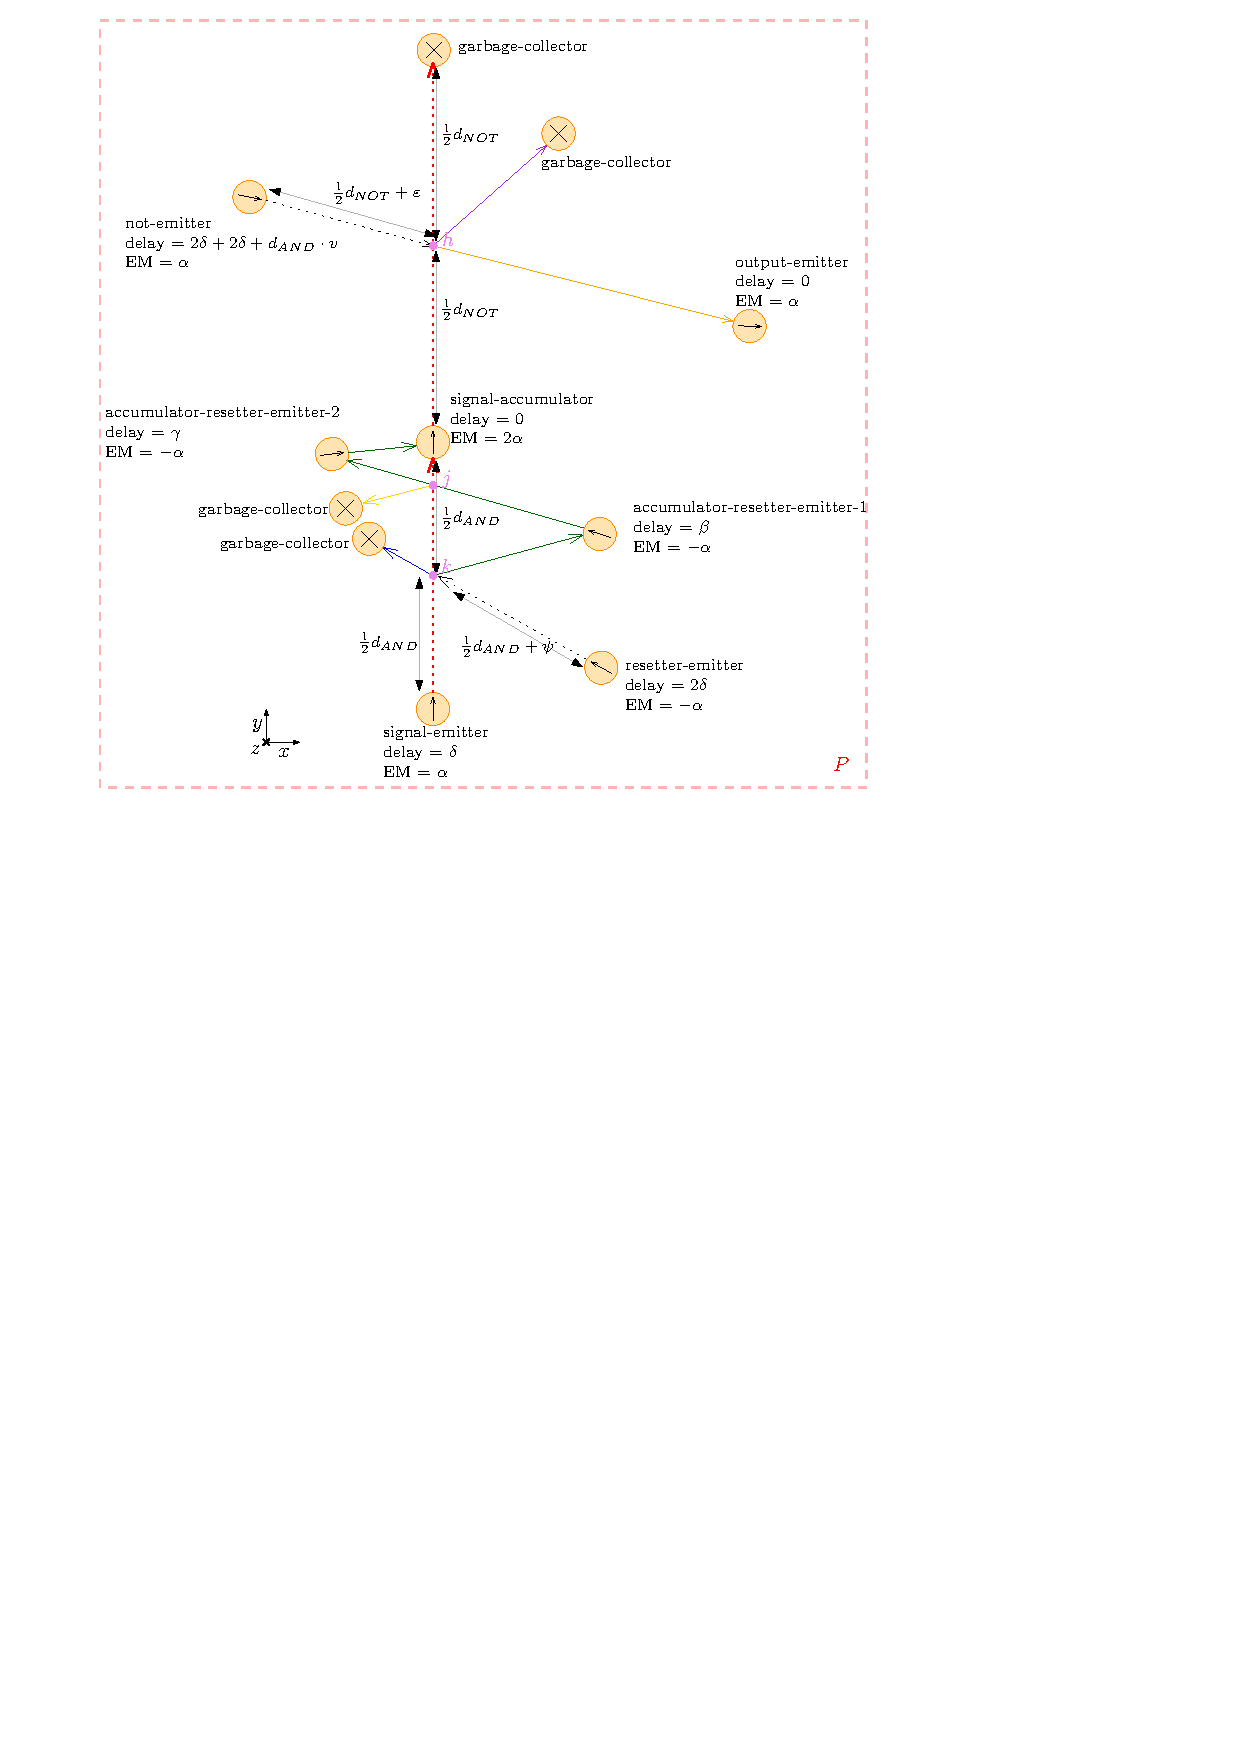
\includegraphics{figures/nand_with_interfaces_v6.pdf}
    \caption{Construction of a NAND-gate in \nenwin as used by the proof of Lemma \ref{lemma:nand_with_iface}. The axes of spatial coordinates $x$ and $y$ are parallel to the place $P$. For each MarbleEmitterNode, the emit-delay and the mass of the emitted marble (EM, 'Emitted Mass', for short) have been denoted. MarbleEmitterNodes are marked with an arrow that indicates the direction of the velocity of the Marble they can emit, and the MarbleEaterNodes (that is not also an EmitterNode) has been marked with a cross. Note that the distances between particles and the radii of the Nodes are not to scale.}
    \label{fig:nand_with_iface}
\end{figure}

\subsection{Tunnel}

Using the the threshold-gravity attraction function \eqref{eq:tresholdgrav}, is it possible to construct an architecture within a rectangular region that can 'steer' a Marble to any other side of the rectangle, and such that it does not interfere with the architecture outside the rectangle. This is proven in the lemma below. The result can be used as a black box in other proofs to 'tunnel' Marbles from one location to another.

\begin{lemma}[Tunnel] \label{lemma:tunnel}
    Let $R = [x_0, x_1] \times [y_0, y_1]$ be a rectangle in $\mathbb{R}^2$. Let $R$ be free of attraction forces from Nodes and Marbles not in $R$. Let $m$ be a Marble with nonzero mass that enters (not only intersects) $R$ via an edge $l$. Then for any point $p = (x_e, y_e)$ on the edges of $R$ that are not $l$, there exist finite numbers $\epsilon, \theta \in \mathbb{R}$ and a finite set of Nodes such that when placed in $R$, $m$ leaves $R$ via $p$.
\end{lemma}
\begin{proof}

    Without loss of generality, assume that $l$ is parallel to the $x$ axis, so all points on $l$ have $x$ coordinates in $[x_0, x_1]$, and the same $y$ coordinate $y_l$. Let $q = (x_q, y_l) \in l$ be the point where $m$ enters $R$.
    
    Let $h$ be the line segment between $q$ and the point $k$, where $k$ is the point where $m$ would have left $R$ if there were no other particles in $R$. Clearly $m$ would move through $R$ in a straight line segment if $R$ were free of other particles, as $R$ is free of forces from particles outside $R$, and hence $m$ would have 0 acceleration. Hence $k$ exists.
    
    If $x_0 < x_q < x_1$, then it is possible to place a Node $n$ with threshold gravity at threshold $\theta + \epsilon$, $\theta, \epsilon > 0$ at $(x_n + \theta, y_n) \in R$ such that the entire attraction field of $n$ is in $R$, $(x_n, y_n) \in h$, $(x_n, y_n) \neq q$ and $0 < \theta \in \mathbb{R}$. If we set $n.mass \leftarrow 0$, then $m$ will leave $R$ at $h$. 
    
    If we make the magnitude of $n.mass$ greater, and set $\sgn{n.mass} \leftarrow \sgn{m.mass}$, and hence the Node's attraction will change $m$'s course more towards the positive $x$ direction; by correct adjustment of $\theta$ and $n.mass$ can clearly adjust the strength of the acceleration and the duration, and hence can steer $m$ to leave $R$ at any point $(x_e, y_e)$ with $x_e > x$ on one of the non-$l$ edges of $R$.
    
    In a similar way, if we set $\sgn{n.mass} \leftarrow -1 \cdot \sgn{m.mass}$ and place $n$ at $(x_n - \theta, y_n) \in R$ instead, then we can steer $m$ to end up any point $(x_e, y_e)$ with $x_e < x$ on on of the non-$l$ edges of $R$.
    
    % If $x_q = x_0$ or $x_q = x_1$, then we can add a second node $n'$ at $(x_q + \theta', y_q)$ or $(x_q - \theta', y_q)$ respectively, with a threshold $\epsilon'$ much smaller than $\theta$. If we would not add a node $n$, then clearly $m$ would exit $R$ at a point $k = (x_k, y_k) \in R$ such that $x_0 < x_k < x_1$. Then let $h$ be the line segment between $q$ and $k$, and we can proceed the proof in a similar way as the case  $x_0 < x_q < x_1$.
    
    If $x_q = x_0$ or $x_q = x_1$, we can use the requirement that $m$ enters $R$, which implies that:
    \begin{enumerate}
        \item If $x_q = x_0$, then the $x$-component of $m.vel$ must be positive, otherwise $m$'s path would only intersect $R$ (move parallel to an edge or only pass the point $q$ no other point of $R$), but not enter it.
        \item If $x_q = x_1$, then the $x$-component of $m.vel$ must negative positive, by a similar argument.
    \end{enumerate}
    In both cases $k$ and $h$ will be well defined, and the construction as of the case $x_0 < x_q < x_1$ can be used.
\end{proof}

See \ref{fig:tunnel} for a visualization of the construction of the proof. 

A conceptually much simpler, but less efficient, method of implementing a 'tunnel' would be to use MarbleEmitterNodes and Marbles, both with 0 Node-attraction and Marble-attraction, in a region of the simulation where no external forces apply: here the Marbles can travel in straight lines between the MarbleEmitterNodes, which provides a method of controlling the movement of Marbles in a sufficiently simple way that it can be designed by hand. One major advantage of this method is that delays can be added to the MarbleEmitterNodes: this way it can be precisely regulated when a Marble will reach the end of the 'tunnel'. Also the velocity magnitude and direction of the resulting Marble emitted by the last MarbleEmitterNode can easily be adjusted.

\begin{figure}[h]
    \centering
    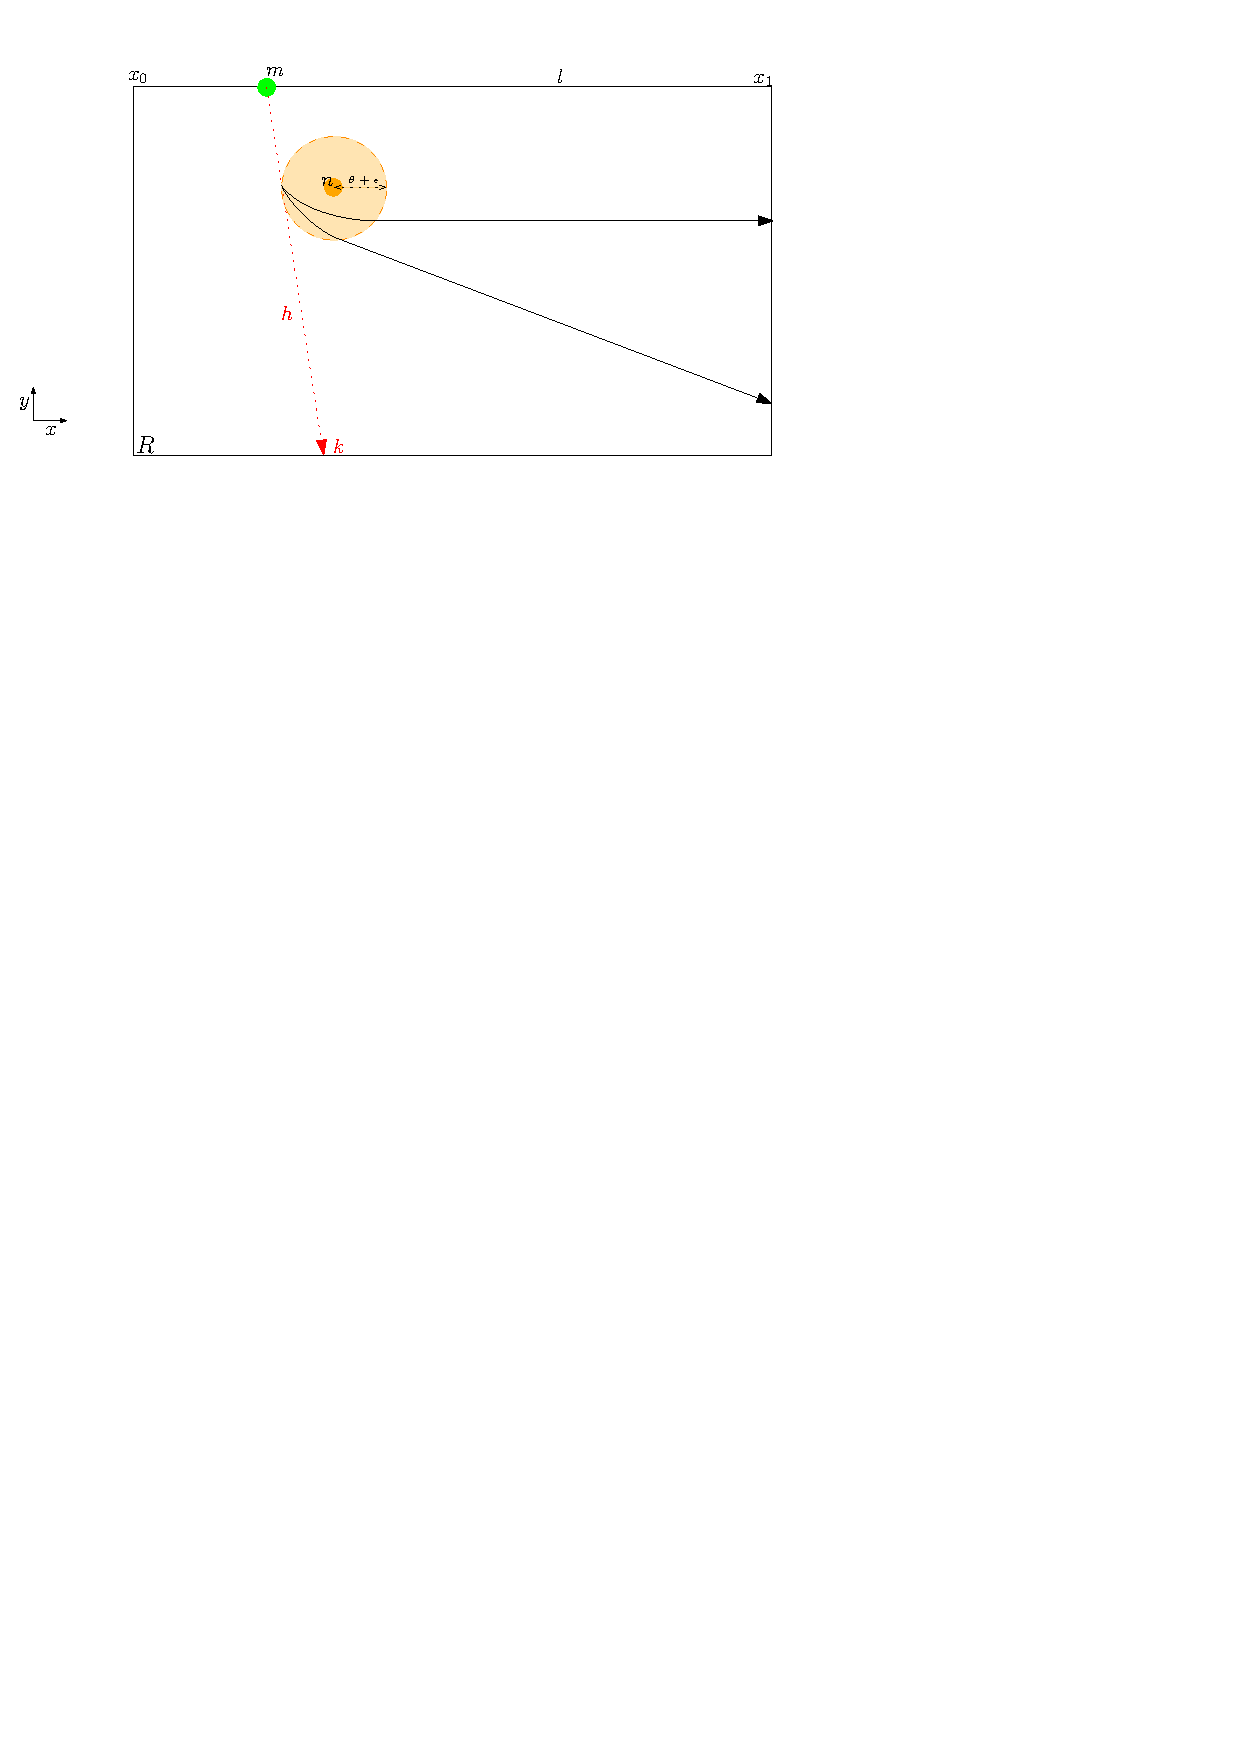
\includegraphics{figures/tunnel_v2.pdf}
    \caption{Construction as used in the proof of Lemma \ref{lemma:tunnel}. The horizontal top edge represents $l$, bounded by $x$-positions $x_0$ and $x_1$. $m$ is the Marble, depicted at the position where it intersects the rectangle $R$ first. The red line represents the path of $m$ if there would be no Node in $R$. The orange point is the node $n$, and the radius of its threshold function has been drawn in transparent orange. Note that $n$ is $\theta$-distance away from $h$, horizontally, hence the radius of the attraction will overlap a little with $h$, which ensures that the movement of $m$ can be influenced by $n$. The black lines represent possible paths trough $R$ of $m$ for two different mass-values of $n$.}
    \label{fig:tunnel}
\end{figure}

\subsection{Bit register}
\nenwin can simulate a single-bit register (i.e. an off-on memory cell).
We present an architecture, for which we can prove the following properties:
\begin{enumerate}
    \item It is possible to read the 0 state
    \item It is possible to read the 1 state
    \item It is possible to set the bit to 0
    \item It is possible to set the bit to 1
\end{enumerate}
The register will be operated by sending a Marble to one of 3 (there is one for reading, one for writing and one for erasing the bit) MarbleEmitterNodes at the edge of the bit. The output will result in a Marble occurring at one of two specific locations that depend on the bit state. This Marble could from there be redirected, or be consumed by a MarbleEaterNode. In the provided architecture the '0-reader' and the '1-reader' are MarbleEaterNodes used at these locations, but for different purposes different elements could be placed here.

\subsubsection{Architecture}
We define the bit architecture $\B$, implemented in $\mathbb{R}^3$ as follows:
\begin{itemize}
    \item Let $P$ be a two-dimensional hyperplane in $\mathbb{R}^3$.
    \item At a specific position in $P$, we create the center of the bit (the 'bit-position'): in the '1' state, this position is occupied by a specific 'bit-Marble', but empty in the '0' state.
    \item A 'bit-emitter' MarbleEmitterNode is placed along the line $l$, which runs though the bit position orthogonal to $P$. We give this MarbleEmitterNode a radius such that the edge of the radius is an infinitesimal distance from the bit position. The Marble that it can emit is the bit-Marble at the bit position.
    \item A 'signal-emitter' MarbleEmitterNode, that is placed at a distance from the bit position in $P$, with a radius sufficiently small not to contain the bit position. The threshold distance is also smaller than the distance from this signal-emitter to the bit-position.
    \item A 'signal-Marble' that can be emitted by the signal-emitter. This Marble has a positive velocity in the direction from the signal-emitter toward the bit-emitter, and is used to pass an external 'write'-signal received by the signal-emitter to the bit-emitter. It has the same mass as the bit-Marble.
    \item Let $\varepsilon \in \mathbb{R}$ be a small yet finite positive number.
    \item A 'read-emitter' MarbleEmitterNode, that is like the signal-emitter also placed in $P$ with a radius and a threshold sufficiently small not to interfere with the bit position. However, it is placed on a different position than the signal-emitter. 
    \item A '0-reader' MarbleEaterNode that is placed in $P$ on the opposite side of the bit position as the read-emitter, but such that the line between the 0-reader and the read-emitter is a distance $\varepsilon$ from the bit position. The radius of this Node can be infinitesimally small, and the threshold distance of its attraction is set to 0.
    \item A 'read-Marble' that can be emitted by the read-emitter, that has an opposite side as the bit-Marble (and hence is repelled by the bit), and a Marble-stiffness of 0. It has a velocity vector in the direction from the read-emitter towards the 0-reader.
    \item A '1-reader' MarbleEaterNode, that is placed in $P$ at an equal distance from the bit-position as the '0-reader', but located such that it will catch the read-Marble if it is repelled by the bit-Marble: it will be proven below that this is not the same location as that of the 0-reader. The radius and the threshold distance have the same values as in the 0-reader.
    \item An 'eraser-emitter' MarbleEmitterNode, similar to the signal-emitter, but at a different position. 
    \item A 'garbage-collector' MarbleEaterNode with similar properties as the 0-reader and the 1-reader, but located exactly on the line running from the eraser-emitter to the bit-position, on the opposite side of the bit-position as the eraser-emitter (this is also in $P$). This Node solely functions to delete Marbles.
    \item An 'eraser-Marble' that can be emitted from the eraser-emitter, with a velocity in the direction from the eraser-emitter towards the bit-position (and hence also towards the garbage-collector). The mass of this eraser-Marble will have the opposite sign as the bit-Marble, and it will have a Node- and Marble-stiffness of 1. The gravity threshold distance of this eraser-Marble is nonzero.
\end{itemize}

The Nodes defined above can all be placed in $\mathbb{R}^3$, on different positions while satisfying their description. All Nodes and Marbles defined above, except the bit-emitter, are placed in $P$ \footnote{It is also possible to place the bit-emitter in $P$, but this would lead to more complex proofs as we need to ensure that it will not interfere with any Marble moving though $P$.}. 

Note that $\B$ should be placed in a region of $\mathbb{R}^3$ where no external forces (except for the Marble that activates reading/writing/erasing) apply, and that when using the threshold gravity function \ref{eq:tresholdgrav}.

The particles of $\B$ and their important properties have been summarized in Table \ref{table:bit}.

\begin{table}[h]
    \begin{tabular}{l|l|l|l|l}
    \textbf{Particle} & \textbf{Type} & \textbf{Mass sign} & \textbf{Marble-stiffness} & \textbf{Marble-attraction} \\ \hline
    bit-Marble        & Marble            & - & 0 & 1 \\
    bit-emitter       & MarbleEmitterNode & 0 &   &   \\
    signal-emitter    & MarbleEmitterNode & 0 &   &   \\
    signal-Marble     & Marble            & - &   &   \\
    read-emitter      & MarbleEmitterNode & 0 &   &   \\
    0-reader          & MarbleEaterNode   & + &   &   \\
    reader-Marble     & Marble            & + & 0 & 0 \\
    1-reader          & MarbleEaterNode   & + &   &   \\
    eraser-emitter    & MarbleEmitterNode & 0 &   &   \\
    garbage-collector & MarbleEaterNode   & 0 &   &   \\
    eraser-Marble     & Marble            & + & 1 & 1
    \end{tabular}
    \caption{Summary of the particles in $\B$, with their most important attributes. 
    Irrelevant values have been omitted: the bit can be made to work for multiple values of these variables. For the mass only the sign and not the magnitude has been recorded, except where the mass is 0. Note that it may not be strictly required to make those particles mass-less, but it simplifies the proof.}
    \label{table:bit}
\end{table}


\begin{figure}
    \centering
    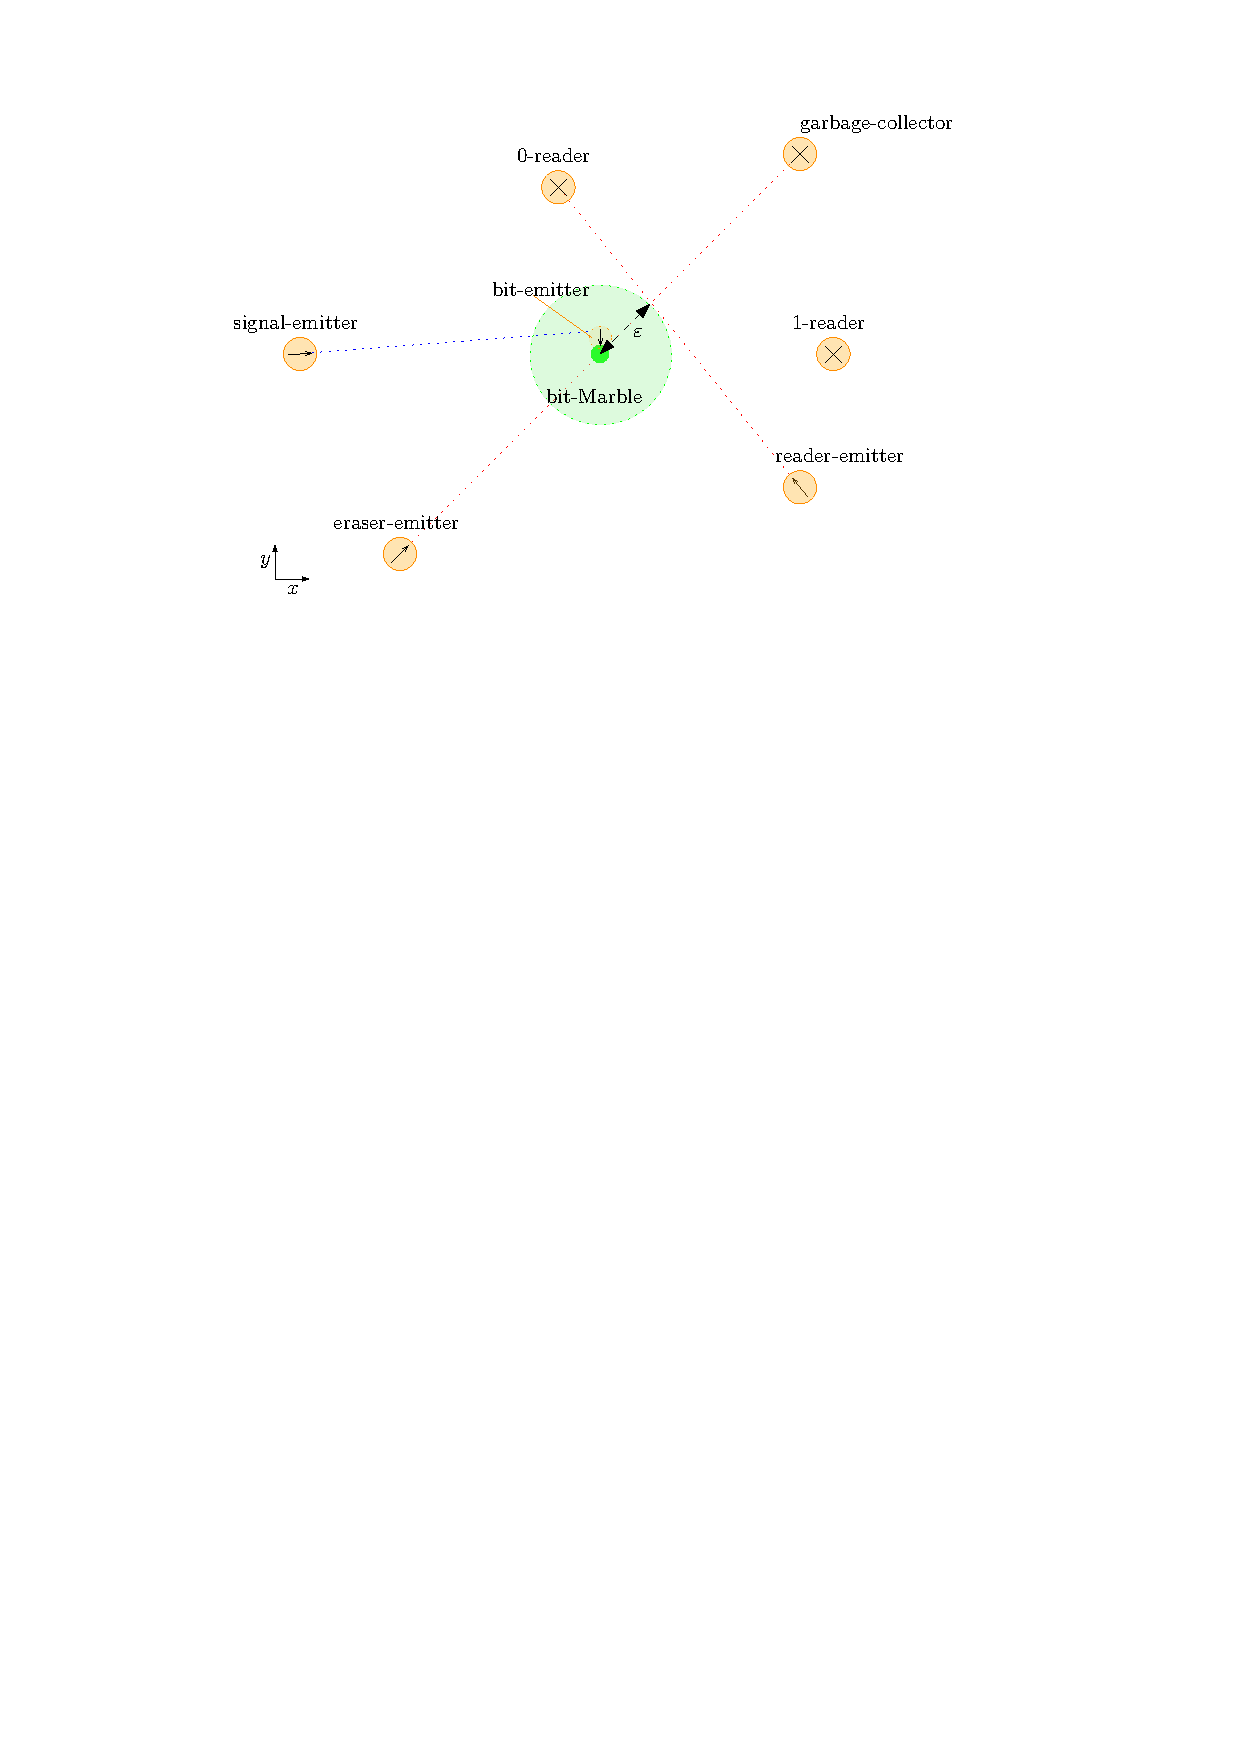
\includegraphics{figures/bit_base.pdf}
    \caption{A visualization of the bit-register architecture $\B$, as projected on a 2-dimensional image. Nodes are drawn in orange, and MarbleEmitterNodes bear an arrow that point in the direction of the velocity of the Marble they can emit. The Bit-Marble is drawn in green, with the threshold-gravity-radius drawn in light-green. Note that the distances and sizes are not necessary to scale.}
    \label{fig:bit_architecture}
\end{figure}

Let $\gamma \subseteq \mathbb{R}^3$ denote the smallest continuous cuboid region in $\mathbb{R}^3$ in which $\B$ has influence (i.e. all particles of $\B$ and all their attraction fields are contained in $\gamma$). 

\begin{lemma}[Reading state 0]
    An external Marble can trigger architecture $\B$ to increase the output of the 0-reader by 1 if the bit register is in the 0-state. After this operation, $\B$ will be in the same state as it started except for the value of the 0-reader.
    \label{lemma:0-reader}
\end{lemma}
\begin{proof}
    Consider an external Marble that enters $\gamma$ at the facet of $\gamma$ that is closest to the reader-emitter, and let this Marble have velocity that moves it in a straight line to the reader-emitter. If this Marble has the correct mass, then the reader-emitter will emit a reader-Marble. This reader-Marble has an initial velocity in the direction of the 0-reader, by design of $\B$. Since there is no bit-Marble to alter its course of motion (since the bit is in state 0) nor any other attraction along its way, it will arrive at the 0-reader. 
    
    Note that the reader-Marble cannot intersect the radius of the bit-emitter, since the bit-emitter does not intersect the plane $P$, in which the reader-Marble remains its entire existence (it moves along the line from the reader-emitter to the 0-reader. These two Nodes are in $P$, and therefore this entire line is in $P$).
    
    Clearly, no particles that existed before the external Marble entered $\gamma$ have been changed during this operation, except for the state of the 0-reader.
\end{proof}

\begin{lemma}[Reading state 1]
     There exists a location for the 1-reader, a value for $\varepsilon$, a mass value and a gravity threshold value for the bit-Marble, such that an external Marble can trigger architecture $\B$ to increase the output of the 1-reader by 1, if the bit register is in the 1-state. After this operation, $\B$ will be in the same state as it started except for the value of the 1-reader.
     \label{lemma:1-reader}
\end{lemma}
\begin{proof}
    As in Lemma \ref{lemma:0-reader}, an external Marble can cause the reader-emitter to emit a reader-Marble. Since the state of the bit is 1, there is a bit-Marble at the bit-position. Now we can adjust $\varepsilon$ the threshold of the bit-Marble's gravity such that the path of the reader-Marble will intersect the attraction field of the bit-Marble at its boundary. Let $p$ the point where this boundary and the line between the reader-emitter and the 0-reader (which define $\varepsilon$) intersect. 
    
    The direction of movement the reader-Marble will not be altered form its starting velocity until it reaches point $p$. Since the mass of the bit-Marble is by construction of the opposite sign as that of the reader-Marble, and since the reader-Marble does not attract Marbles but is attracted by them (by construction), only the acceleration of the reader-Marble will be affected. The reader-Marble will be accelerated in the same direction as the line segment between the bit-position and $p$, and this direction is orthogonal to the direction reader-Marbles initial velocity. 
    
    Since the reader-Marble intersects only shortly this acceleration is present only one instant of time. However, if the mass of the bit-Marble is of sufficient magnitude, it will change the direction of the velocity of the reader-Marble significantly. The new direction of this velocity is not the opposite of the original direction, as the acceleration was orthogonal to the original velocity of the reader-Marble. Hence the reader-Marble will not arrive at the reader-emitter (which requires the opposite direction as the original velocity of the reader-Marble had) nor the 0-reader (which requires the original direction). 
    
    Note that the reader-Marble cannot intersect the radius of the bit-emitter, since the bit-emitter does not intersect the plane $P$, in which the reader-Marble remains its entire existence.
    (as in Lemma \ref{lemma:0-reader}, the initial path of the reader-Marble is in $P$. Since $p$ is on the line between the reader-emitter and the 0-reader, $p$ is in $P$ as well. Now since the bit-position is also in $P$, the acceleration vector is also in $P$. The resulting velocity of the reader-Marble is a linear combination of its prior velocity and the acceleration, which are both vectors in $P$, hence the reader-Marble remains in $P$.)
    
    The 1-reader can be positioned along the line from the reader-Marble in the new direction of the Marble's velocity, and then the reader-Marble will eventually be consumed by the 1-reader.
\end{proof}

\begin{lemma}[Writing bit]
    An external Marble can trigger architecture $\B$ when in state 0 (no bit-Marble present) to enter state 1 (with a bit-Marble present), without any other particle in $\B$ being affected after completion.
    \label{lemma:writing}
\end{lemma}
\begin{proof}
    Let the external Marble enter $\gamma$ in the point closest point of the closest facet of $\gamma$ to the signal-emitter, with a velocity the direction of the line from that point to the signal-emitter. Then this Marble will be consumed by the signal-emitter, and if it of sufficient mass it will trigger the signal-emitter once to emit a signal-Marble.
    
    The signal-Marble is configured (by construction of $\B$ to have a velocity in the direction of the signal-emitter towards the bit-emitter, and since it is not attracted by Marbles or Nodes, nor does any Eater- or EmitterNode block its path, it will eventually be consumed by the bit-emitter. Consequently, the bit-emitter creates a single bit-Marble.
\end{proof}

\begin{lemma}[Erasing bit]
    An external Marble can trigger architecture $\B$ when in state 1 (a bit-Marble present) to enter state 1 (no bit-Marble present), without any other particle in $\B$ being affected after completion, except for the mass stored in the garbage-collector.
    \label{lemma:erasing}
\end{lemma}
\begin{proof}
    Let the external Marble enter $\gamma$ in the closest point of the closest facet to the eraser-emitter, with a velocity in the direction of the line from this point towards the eraser-emitter. The Marble will be consumed by the signal-emitter, and if the external Marble had enough mass, an eraser-Marble will be emitted in the direction of the bit position. Note that the eraser-Marble has both a Node- and Marble-stiffness of 1, hence no attraction force will affect its acceleration. Hence it will travel in a straight line with constant velocity.
    
    The eraser-Marble has a Marble-stiffness of 1, and since the bit-Marble has a Marble-stiffness of 0, the bit-Marble's motion will be affected when the eraser-Marble nears the bit-Marble. Since the mass of the eraser-Marble is of the opposite sign as that of the bit-Marble, it will repel the bit-Marble, which will be accelerated in the same direction as the eraser-Marble is moving. Now we can adjust the masses of the bit-Marble and the eraser-Marble such that the repellent force is strong enough the accelerate the bit-Marble to the same or a higher velocity as the eraser-Marble before the eraser-Marble reaches the bit-position: this will guarantee that the eraser-Marble will not 'take-over' the bit-Marble and repel it in the other direction.
    
    Now both Marbles will travel in the direction of the line from the eraser-emitter to the bit-position. By construction of $\B$, the garbage-collector is also on this line and on the other side of the bit-position as the eraser-emitter. Therefore both Marbles will eventually enter the radius of the garbage-collector and be absorbed.
\end{proof}

We can summarize the results of Lemma \ref{lemma:0-reader}, \ref{lemma:1-reader}, \ref{lemma:writing} and \ref{lemma:erasing} in the following theorem:

\begin{theorem}[Bit register]
    There exist settings for the parameters of $\B$, and an external Marble $m$ outside of $\gamma$, such that by moving $m$ with the right value of $m.vel$, $m.pos$ and $m.mass$ into $\gamma$:
    \begin{enumerate}
        \item $m$ can trigger the reading of the bit. That is, after sufficient time, if there is a bit-Marble present, the 1-reader's number-of-Marbles-consumed count will increase by 1. If there no bit-Marble present, after sufficient time, the count of the 0-reader will increase by 1. When this count increases, the collection of particles in $\gamma$ and their states are identical to the situation before $m$ entered $\gamma$.
        \item $m$ can cause the creation of a bit-Marble in $\B$ without affecting the state of other particles in $\B$.
        \item $m$ can cause the removal of a bit-Marble in $\B$, when present, without affecting the state of other particles in $\B$ except for the Marbles consumed by the garbage-collector.
        \item Furthermore, $\B$ does not directly affect particles outside $\gamma$.
    \end{enumerate}
\end{theorem}
\begin{proof}
    \begin{enumerate}
        \item Follows from Lemma \ref{lemma:0-reader} and Lemma \ref{lemma:1-reader}.
        \item Follows from Lemma \ref{lemma:writing}.
        \item Follows from Lemma \ref{lemma:erasing}.
        \item The particles in $\B$ are constructed around a finite distance from the bit-position in $\mathbb{R}^3$, use finite radii and are using the threshold gravity as attraction function with a finite threshold. Hence in each direction from the bit-position, there is a distance that surpasses the influence of attraction functions, radii and positions of particles. By construction of $\gamma$, the minimum value of this distance either defines a facet of $\gamma$ or is interior to $\gamma$. Hence outside $\gamma$, $\B$ cannot affect any particle directly.
    \end{enumerate}
\end{proof}

\subsection{Clock and divider}
Implementing a clock in \textsc{Nenwin} is trivial: a MarbleEmitterNode with a large amount of \texttt{stored\_mass} (e.g. a value of $\infty$) and a positively-valued delay will already periodically emit a Marble. Since Marbles are used to represent signals, this suffices to implement a periodical signal-creating device. However, the signal needs to reach multiple components after a sufficiently large delay, and a single Marble can be absorbed only once. Multiple clocks could be used, but a solution that reduces the amount of clocks needed is to use 'splitters':
\begin{lemma}
    Given a finite region $R \subset \mathbb{R}^x$ ($x \geq 2$) in a \textsc{Nenwin} architecture with no external forces, it is possible to construct an architecture in $R$ such that when a Marble $m$ with mass $\alpha$ enters $R$ at a designated point $q$ at $t_0$, that this causes any fixed amount $n \geq 0$ Marbles to be emitted from $R$ with velocities in different directions, at a time $t_0 < t_1 < \infty$. This architecture in $R$ will not emit Marbles or exerts forces outside $R$ otherwise.
    \label{lemma:splitter}
\end{lemma}
\begin{proof}
    The case when $n = 0$ is trivial, a single MarbleEaterNode positioned in $R$ with 0 Marble- and Node-attraction and a radius that intersects $q$.
    
    For $n \geq 1$, consider the following architecture (where all particles have a Marble- and Node-stiffness of 1 unless denoted otherwise) (see also Fig. \ref{fig:splitter}):
    \begin{itemize}
        \item Let $P$ be a rectangle on a plane though $R$ with maximal surface area.
        \item A 'signal-emitter': a MarbleEmitterNode, positioned such in $P$ with such a radius that the border of the radius intersects the border of $R$. It has a delay of $\delta$.
        \item Let $l$ be the ray parallel to $P$ that starts in the signal-emitter and that intersects the center of $P$.
        \item A 'signal-Marble': the Marble that can be emitted by the signal-emitter. Let it have a mass of $\alpha$ and a velocity direction parallel to the $l$ (towards the centre of $P$) and a velocity magnitude of $v_{signal}$. 
        \item Two 'locker-Nodes': two Nodes with the same negative mass, placed in $P$, both on a line $l'$ in $P$ orthogonal to $l$ that also intersects the center of $P$, each at a different side of $l$, each at an equal distance from $l$. Their threshold distance of their attraction functions have the same positive value. Let these Nodes have a Marble-attraction of 0 and a Node-attraction of 1.
        \item A 'moving-emitter': a MarbleEmitterNode initially placed with a specific positive mass and a specific velocity $v_{Node}$ at a specific point $p'$ on $l'$ where the distance to the clostest locker-Node is $d + \varepsilon$, such that it will be deaccelerated by locker-Node untill it halts on a point $p$ at a distance $d$ from this locker-Node, and will reverse its direction when it is a distance $d$ from that locker-Node: hence $p'$ is an extreme point of the harmonic motion this moving-emitter will show. Let $\delta$ be the period of the harmonic motion. Let the moving-emitter have a delay of $\frac{delta}{2\cdot n}$. Let this Node be the only Node in $R$ with a Marble- and Node-stiffness both of 0.
        \item Let $v_{signal}$ equal $\frac{\frac{\varepsilon}{v_{Node}}}{z}$  where $z$ is the smallest component parallel to $l$ of the distance form the point where the signal-Marble is emitted to the border of the radius of the moving-emitter (which equals the distance from the point where the signal-Marble is created to the closest border of the signal-emitter when the latter is in the point $p$).
        \item $n$ 'output-emitters' named $O_1, O_2, \dots, O_n$, placed in $P$ on the opposite side of $l'$ as the signal-emitter is, such that at a time $t_0 + i \cdot \frac{\delta}{2 \cdot n} \mod \delta$ the moving-emitter is in a position where a line-segment $k_i$ exists in $P$ that is parallel to $l$ and intersects both the moving-emitter and $O_i$ for $1 \leq i \leq n$, and such that the position and radius have that the border of their radius intersect the border of $R$. 
        \item Let the 'split-Marbles' be the Marbles emitted by the moving-emitter with a mass of $\frac{\alpha}{2}$ and a velocity parallel to $l$ (away from the center of $P$).
    \end{itemize}
    Note that the distance between each line segment $k_i$ and $k_j$, $1 \leq i < j \leq n$ is not necessarily equal as the moving-emitter does not have a constant velocity and hence does not travel a fixed amount of distance in the same time span.
    
    Now if $m$ is consumed by the signal-emitter at time $t = t_0$, it will emit a signal-Marble. By construction of the moving-emitter, it will be at point $p$ at time $t = t_1 = t_0 + \frac{\varepsilon}{v_{Node}}$. But by construction, this is also the time required by the signal-Marble to travel to the point where it would be consumed by the moving-emitter if it were at point $p$. Since the moving-emitter is at point $p$, it will consume the Marble. By definition of point $p$, this is the point where the direction of the velocity of the moving emitter reverses in direction. So at time $t = t_1 + \frac{delta}{2\cdot n}$, by construction, the moving-emitter will be positioned on $k_1$. Since its first delay has been satisfied, it will emit the first split-Marble, which is created in such a position where it will move in a direct line to $O_1$. Now the \texttt{stored\_mass} of the moving-emitter is $\alpha - \frac{\alpha}{n}$. The same process is repeated for $O_2$, $O_3$, \dots, $O_n$. Let $\hat{p}$ the point that is the image of $p$ when mirroring $p$ in $l$ on $P$. Because of the harmonic motion, the moving-emitter will reverse its direction again at point $\hat{p}$, but at this point its \texttt{stored\_mass} is 0. Hence on the 'return trip' to $p$ it will not emit any Marble. Now each of the output-emitters $O_1$, $O_2$, \dots, $O_n$ has received exactly one split-Marble. Since each of the output-emitters intersects the boundary of $R$, each can create an output Marble outside $R$ with a mass of $\frac{\alpha}{n}$, each in a different direction.
    
    At time $t = \delta$, the moving-emitter is at point $p'$ again with a \texttt{stored\_mass} of 0, and if the velocity of the split-Marbles is large enough and the delay of the output-Marbles is small enough, all particles in $R$ will be in the exact same state as at $t_0$.
    
    It remains to prove the harmonic motion of the moving-emitter. Note that if the threshold-distance of the locker-Nodes is at least as far as the distance to the other locker-Node, that the situation is equivalent to the physical model of simple harmonic motion under Newton's model of gravity \cite{principia}. It is beyond the scope of this report to prove simple harmonic motion, but the reader is referred to, for example, \cite{uni_physics}.
\end{proof}
Note that the NAND-gate requires both positively and negatively massed Marbles as 'power' from the clock to operate. This can be implemented by using two synchronized MarbleEmitterNodes, one which emits positively massed Marbles, and the other negatively massed Marbles.

\begin{figure}[h]
    \centering
    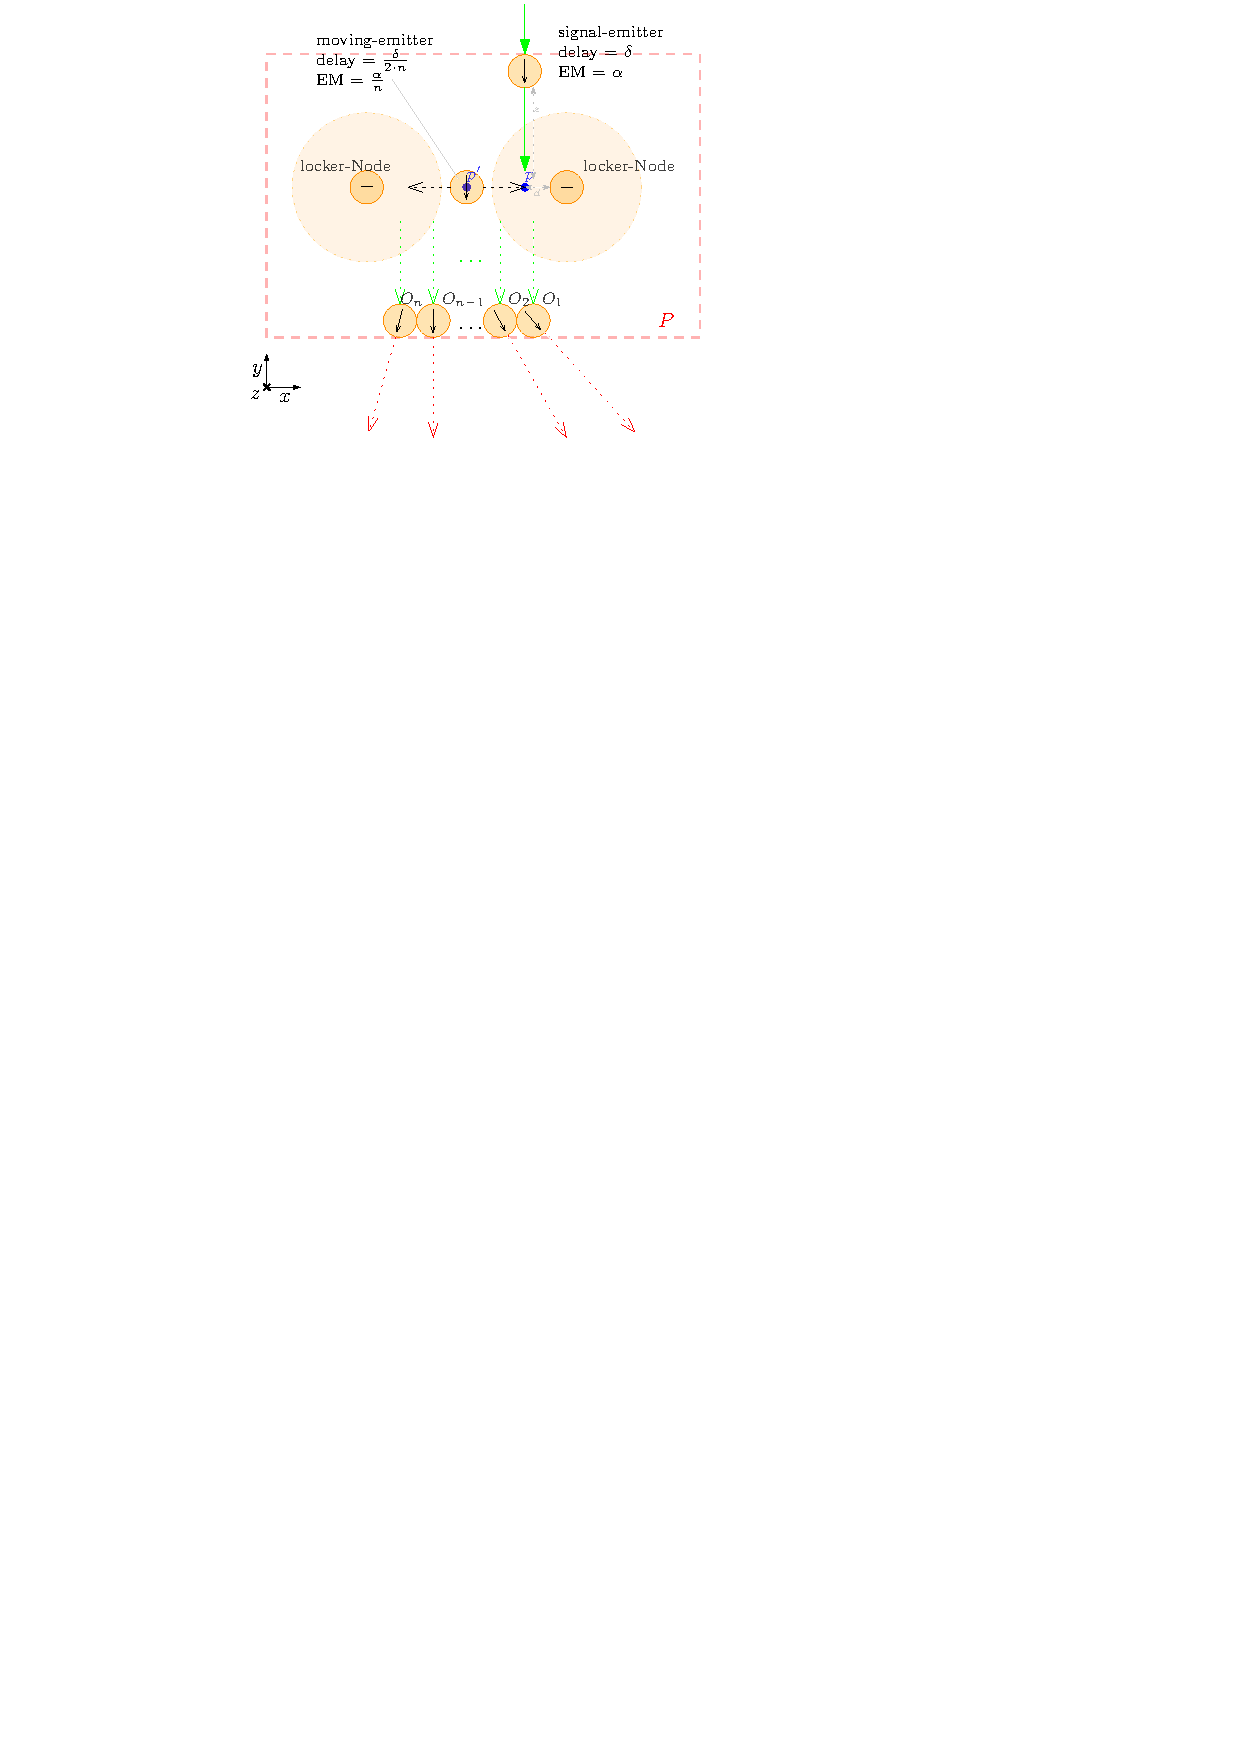
\includegraphics{figures/splitter_v4.pdf}
    \caption{Construction as used in the proof of Lemma \ref{lemma:splitter}. The naming of objects is analogous with the proof. The black dotted arrows denote the directions of velocity of the moving-emitter, the red dotted arrows denote possible directions of velocity of the output Marbles, the green dotted arrows denote the last segment of the movement of the split-Marbles that are released by the moving-emitter, and the continuous green arrows denote the movement of the input-Marble and the signal-Marble.}
    \label{fig:splitter}
\end{figure}



\subsection{Section conclusion}
It is beyond the scope of this report to describe a complete implementation of a CPU in \textsc{Nenwin}, but sufficient important components have been described to abstract from the implementations of components, and reason on the (sequential) logical circuit level of abstraction. How to design a CPU with such circuits has been described in many sources, such as \cite{comp_architecture} and \cite{comp_org_design}.

\clearpage
    
    \section{Training}
    As shown in the previous section, \textsc{Nenwin} is capable to simulate a CPU. Given that the RAM model is Turing complete, \textsc{Nenwin} is a Turing complete computational method as well. However, \textsc{Nenwin} has a very dynamic nature with complex interactions between particles, especially for larger architectures. This makes it unpractical to design architectures manually; automated optimization, or 'training', is needed for any practical application. 

The goal of the training is to set up the architecture of Nodes, such that on a specific input $x \in \mathbb{R}^n$, $n \in \mathbb{N^+}$, given at a point in time $t = t_x$, leads to a desired output $y \in \mathbb{R}^m$, $m \in \mathbb{N^+}$ at a specific time $t = t_y > t_0$. Note that the way $y$ is represented by the \textsc{Nenwin} model can be defined in multiple ways.
    
    \subsection{A first experiment: EaterNodes as output}
    For a classification task it is required that a model can output a prediction.
This prediction can for example simply by a discrete class label,
but also a probability distribution. 
In \nenwin it is straightforward to obtain a one-hot-encoding of discrete class label as output, by using MarbleEaterNodes.
In this case, the output will simply be a vector of integers, 
where each value represents the number of Marbles eaten by each MarbleEaterNode.
The MarbleEaterNodes may be ordered in any arbitrary fix order, as long as, at each point in time $t = t_j$, 
the output can be interpreted as an array with one value for each MarbleEaterNode.

This can be expressed more formally as defining a \textit{cumulative output vector}:
\begin{definition}[cumulative output vector] \label{def:cumul_output_vect}
Given a \nenwin model $M$, then for each point in time $t$, define the \textbf{cumulative output vector} $\vec{M}(t)$ as:
\begin{equation}
    \vec{M}(t)_i \equiv \text{number of Marbles eaten by the $i^{th}$ MarbleEmitterNode at time $t$}
\end{equation}
\end{definition}
Note that $\vec{M}(t)$ is always a vector of nonnegative integers, and at $t = 0$ we have $\vec{M}(0) = \vec{0}$.


\subsection{Loss definition}
The output of the model changes over time, and hence it is practical to define the 'real' output $\hat{\vec{y}}$ as the time-varying output read at a certain point in time. For convenience, call this time $t_{end}$. Then \begin{equation}
    \hat{y} \equiv \vec{M}(t_{end})
\end{equation} Given an expected output $\vec{y}$, the most straightforward way to define the \textit{loss} of the 'real' output $\hat{\vec{y}}$ is to take a measure of difference between $\vec{y}$ and $\hat{\vec{y}}$, such as the Mean Squared Error or the Cross Entropy Loss. However, this approach is not optimizable in all situations, as explained below.

\subsubsection{Classification loss}
Consider an application where a \nenwin model is used to classify an input as one out of $k$ classes. Let each class-prediction be represented by a single MarbleEaterNode. Now since only one class is needed, the output $\hat{\vec{y}}$ can be read when the first Marble is eaten, or when the time $t = t_{max}$. More formally, let 
\begin{equation}
    t_{end} \leftarrow \min \left(\{t \; | \; 1 \leq \norm{\vec{M}(t)}\}\cup \{t_{max}\}\right).
\end{equation}
Now there are three possible cases for the output $\hat{\vec{y}}$ 
(for now, assume only one Marble will be eaten at $t = t_{end}$):
\begin{enumerate}
    \item $\hat{\vec{y}} = \vec{y}$, and the loss can be set to 0.
    \item $t_{end} = t_{max}$ and $\hat{\vec{y}} = \vec{0}$, that is, no Marble has been eaten.
    \item $\hat{\vec{y}} \neq \vec{y}$ (and $\hat{\vec{y}} \neq \vec{0}$).
\end{enumerate}

In case 2, it is expected that a Marble arrived at a specific MarbleEmitterNode $n$. However, there may be multiple Marbles present in the model, hence it is not clear \textit{which} Marble should be eaten by $n$ to achieve the desired output. 
The chosen method to resolve this is choosing the Marble $m$ for which the loss would be smallest.
Intuitively, this method 'blames' the Marble that seems most promising to be eaten by $n$ for the loss.
More formally, define:
\begin{equation}
    L(\hat{\vec{y}}, \vec{y}) = \smashoperator{\min_{m \in Marbles}} \; f(m, n, t_{end}) \label{eq:classification_loss_net}
\end{equation}
where
\begin{equation}
    f(m, n, t) = \big\Vert{n.pos(t) - (m.pos(t) + \mu \cdot m.vel(t))}\big\Vert_2^2, \qquad \mu \in \mathbb{R}_{\geq 0}. \label{eq:classification_loss_one_marble}
\end{equation}
Here $\mu$ is a nonnegative real number that functions as a hyperparameter. 

The rationale behind including the '$+ \mu \cdot m.vel$' term is as follows: 
if only the position of the Marble is optimized, 
then it will be closer to $n$ at $t = t_{end}$, 
but this does not necessary imply it is also closer to being eaten by $n$. 
'Almost being eaten' also requires $m$ to be moving towards $n$!
'$+ \mu \cdot m.vel$' can be seen as a very naive prediction of the future position of $m$. 
The intent of this addition is to make it more likely that 'minimizing the loss function' correlates with 'making $m$ being eaten by $n$'.

$\mu$ could be fixed as a hyperparameter, but this may cause undesired effects when the  magnitude of $m.vel$ changes significantly. For example, if $\norm{m.vel}$ and $\mu$ are both large, then $m.pos + \mu \cdot m.vel$ might be further from $n.pos$ than $m.pos$, even if the direction of $m.vel$ is from $m.pos$ towards $n.pos$ (i.e. the naive prediction \textit{overshoots}). It may be wise to make $\mu$ a function of the magnitude of $m.vel$, e.g. to demand that $\mu \propto \frac{1}{\norm{m.vel}}$.

For case 3, also \eqref{eq:classification_loss_net} can be used for the missing Marble at the expected output MarbleEaterNode encoded in $\vec{y}$. However, there is also another Marble, $m'$, which was eaten by some node $n' \neq n$ (otherwise case 3 would equal case 2 or case 1), where $n'$ is the MarbleEaterNode at the unique index $i$ where $\hat{y}_i = 1$. Since $m'$ is eaten at $t = t_{end}$, $f(m', n', t_{end})$ (using \eqref{eq:classification_loss_one_marble}) is well defined, and the following loss function would penalize $m'$ moving towards $n'$:

\begin{equation}
    L(\hat{\vec{y}}, \vec{y}) = - \frac{1}{f(m', n', t_{end})} + \smashoperator{\min_{m \in Marbles}} \; f(m, n, t_{end})
\end{equation}

The reciprocal $- \frac{1}{f(m', n', t_{end})}$ is used instead of $f(m', n', t_{end})$, 
as the latter will be small in magnitude (considering the Marble was eaten), 
but becomes larger the further $m'$ is away from $n'$. 
But the further $m'$ is away from $n'$, the less $m'$ should be corrected.

It is possible to add scalar weights to each of the two terms 
$- \frac{1}{f(m', n', t_{end})}$ and $\min_{m \in marbles} f(m, n, t_{end})$, 
but this approach has not been explored further.

In summary, the loss $L(\hat{\vec{y}}, \vec{y})$ is defined as:
\begin{equation}
    L(\hat{\vec{y}}, \vec{y}) = \begin{cases}
        0 & \text{if } \hat{\vec{y}} = \vec{y} \\
        - \frac{1}{f(m', n', t_{end})} + \min_{m \in Marbles} f(m, n, t_{end}) & \text{if } \vec{y} \neq \hat{\vec{y}} \neq \vec{0}  \\
        \min_{m \in Marbles} f(m, n, t_{end}) & \text{if } \hat{\vec{y}} = \vec{0}\\
    \end{cases}
    \label{eq:classification_loss_full}
\end{equation}
Where $n$ is the node at the unique index $i$ where $y_i = 1$, $Marbles$ is the set of all Marbles in the model, and $m'$ is \textit{the} Marble eaten by some node $n' \neq n$ in the case $\vec{y} \neq \hat{\vec{y}} \neq 0$.

\subsubsection{Multiple outputs}
Eq. \eqref{eq:classification_loss_full} assumes that at most one Marble will be eaten. 
It is possible that multiple Marbles will be eaten at the same time. 
Especially in simulation this is not unlikely, where discrete finite-sized time steps are taken.

Let $k$ be the number of Marbles eaten at $t = t_{end}$, and let these Marbles be $m_1, m_2, \dots, m_k$. 
Let the corresponding MarbleEaterNodes that ate them be $n_1, n_2, \dots, n_k$. 
Note that these MarbleEaterNodes may not all be distinct, while the Marbles are all unique. 
Let $n$ be the MarbleEaterNode of the correct (expected) output. 
Then we can extend \eqref{eq:classification_loss_full} to:
\begin{equation}
	L_{total}(\hat{\vec{y}}, \vec{y}) = \mathbbm{1}(n\notin \{n_1, n_2, \dots, n_k\}) \cdot \smashoperator{\min_{m \in Marbles}} f(m, n, t_{end}) 
									  - \sum_{i=1}^{k}   \frac{1}{f(m_i, n_i, t_{end})}
\end{equation}
Where $\mathbbm{1}(p)$ equals 1 if the proposition $p$ is true, and 0 if $p$ is false.
In the very specific case that \textit{all} Marbles have been eaten by the wrong Nodes,
the term $\min_{m \in Marbles} f(m, n, t_{end})$ will not be defined. 
It was chosen to simply leave this term out in this case. 
If the penalty for the wrongly eaten Marbles causes sufficient change in the update rule, 
then (in the next iteration, or a few iterations later) 
there will be uneaten Marbles available to 'blame' for not being eaten by the correct MarbleEaterNode.

In other words:
\begin{itemize}
	\item For each wrongly outputted Marble, the wrong-output penalty is added to the loss.
	\item In case the correct output was not included, also the missing-output penalty is added once.
\end{itemize}

Note that this method does not penalize multiple Marbles arriving at the correct output Node, 
which may in some contexts also be undesirable.

\subsubsection{Non-convexity}
Eq. \eqref{eq:classification_loss_full} is not convex. This is not surprising given its relatively complex piece-wise definition. 
%To simplify the notation, define the following extension of Definition \ref{def:cumul_output_vect}:
%
%\begin{definition}[Parametrized cumulative output vector]
%    Let $\vec{M_{\theta}}(t)$ denote the \emph{cumulative output vector} $\vec{M}(t)$ of a \nenwin architecture whose initial particles are described by $\theta$.
%\end{definition}

The following lemma proofs that even optimizing the initial values (which are the initial position, velocity, acceleration and the mass) of particles, keeping the set of particles themselves constant, does not have a convex objective.
\begin{lemma}[Non-convexity of \eqref{eq:classification_loss_full}]
Assuming a constant vector $\vec{y}$, \eqref{eq:classification_loss_full} is not convex, for all \nenwin architectures, in the \emph{initial values} of the particles.
\label{lemma:nonconvexity_loss}
\end{lemma}
\begin{proof}
For simplicity, we proceed with a specific counter-example. 
Consider an architecture with a single Marble $m$, two MarbleEmitterNodes $E_1$ and $E_2$, and a MarbleEaterNode $n$.
Let $\vec{y} = [1]$. 
Let both emitters have such a threshold and such a prototype that if they eat $m$, 
they will emit some new Marble $m'$ that will move towards $n$ and be eaten in $t' < \frac{1}{2}t_{end}$ time. 
Let $m.node\_stiffness = 1$. 
Now position the four initial particles on the vertices of a sufficient large square that their radii do not overlap, 
and $E_1$ and $E_2$ oppose each other. 
Let $A$ be the vertex assigned to $m$. 
The parameter of interest is now the initial velocity of $m$, in particular the \emph{angle} of $m.vel(t_0)$. 
Let the magnitude of $m.vel$ be such that, under constant $\vec{0}$ acceleration and no obstacles, 
$m$ would travel several times the length of an edge of the square. 
Now define the following angles $a_1 < a_2 < \dots < a_7$ of the direction of $m.vel$ (see Fig. \ref{fig:nonconvexity_loss}):
\begin{itemize}
    \item $a_2$: $m.vel$ is directed towards $E_1$, then $E_1$ would emit a Marble which arrives at $n$ before $t = t_{end}$. Hence the loss would be 0.
    \item $a_3$: $m.vel$ is directed towards the center of the edge of the square between $E_1$ and $n$. At $t = t_{end}$, $m$ would still exist and be far from $n$, and hence the loss would be much greater than 0.
    \item $a_4$: $m.vel$ is directed towards $n$ and $m$ will be eaten by $n$ before $t = t_{end}$, the loss will be 0.
    \item $a_5$: $m.vel$ is directed towards the center of the edge of the square between $E_2$ and $n$. The loss of this case is the same as in case 2 (i.e. nonzero).
    \item $a_6$: $m.vel$ is directed towards $E_2$. The loss of this case is 0, by symmetry with case 1.
    \item $a_1$ or $a_7$: $m.vel$ is not directed to the inside of the square, nor parallel or close to parallel to one of the edges, nor to one of the regions within the radii of $E_1$ or $E_2$. The loss will be nonzero as $n$ will not eat any Marble.
\end{itemize}
$\hat{\vec{y}}$ is a function of the initial values of the particles and the angle of $m.vel$ is part of these initial values. The loss in the case of $a_3$ is larger than in the case of $a_2$ or $a_4$ (see also Fig. \ref{fig:nonconvexity_loss_plot}). Clearly this violates the convexity property, and hence \eqref{eq:classification_loss_full} is not convex in the angle of $m.vel$, and hence not in all initial values of the particles.
\end{proof}

\begin{figure}[h]
    \centering
    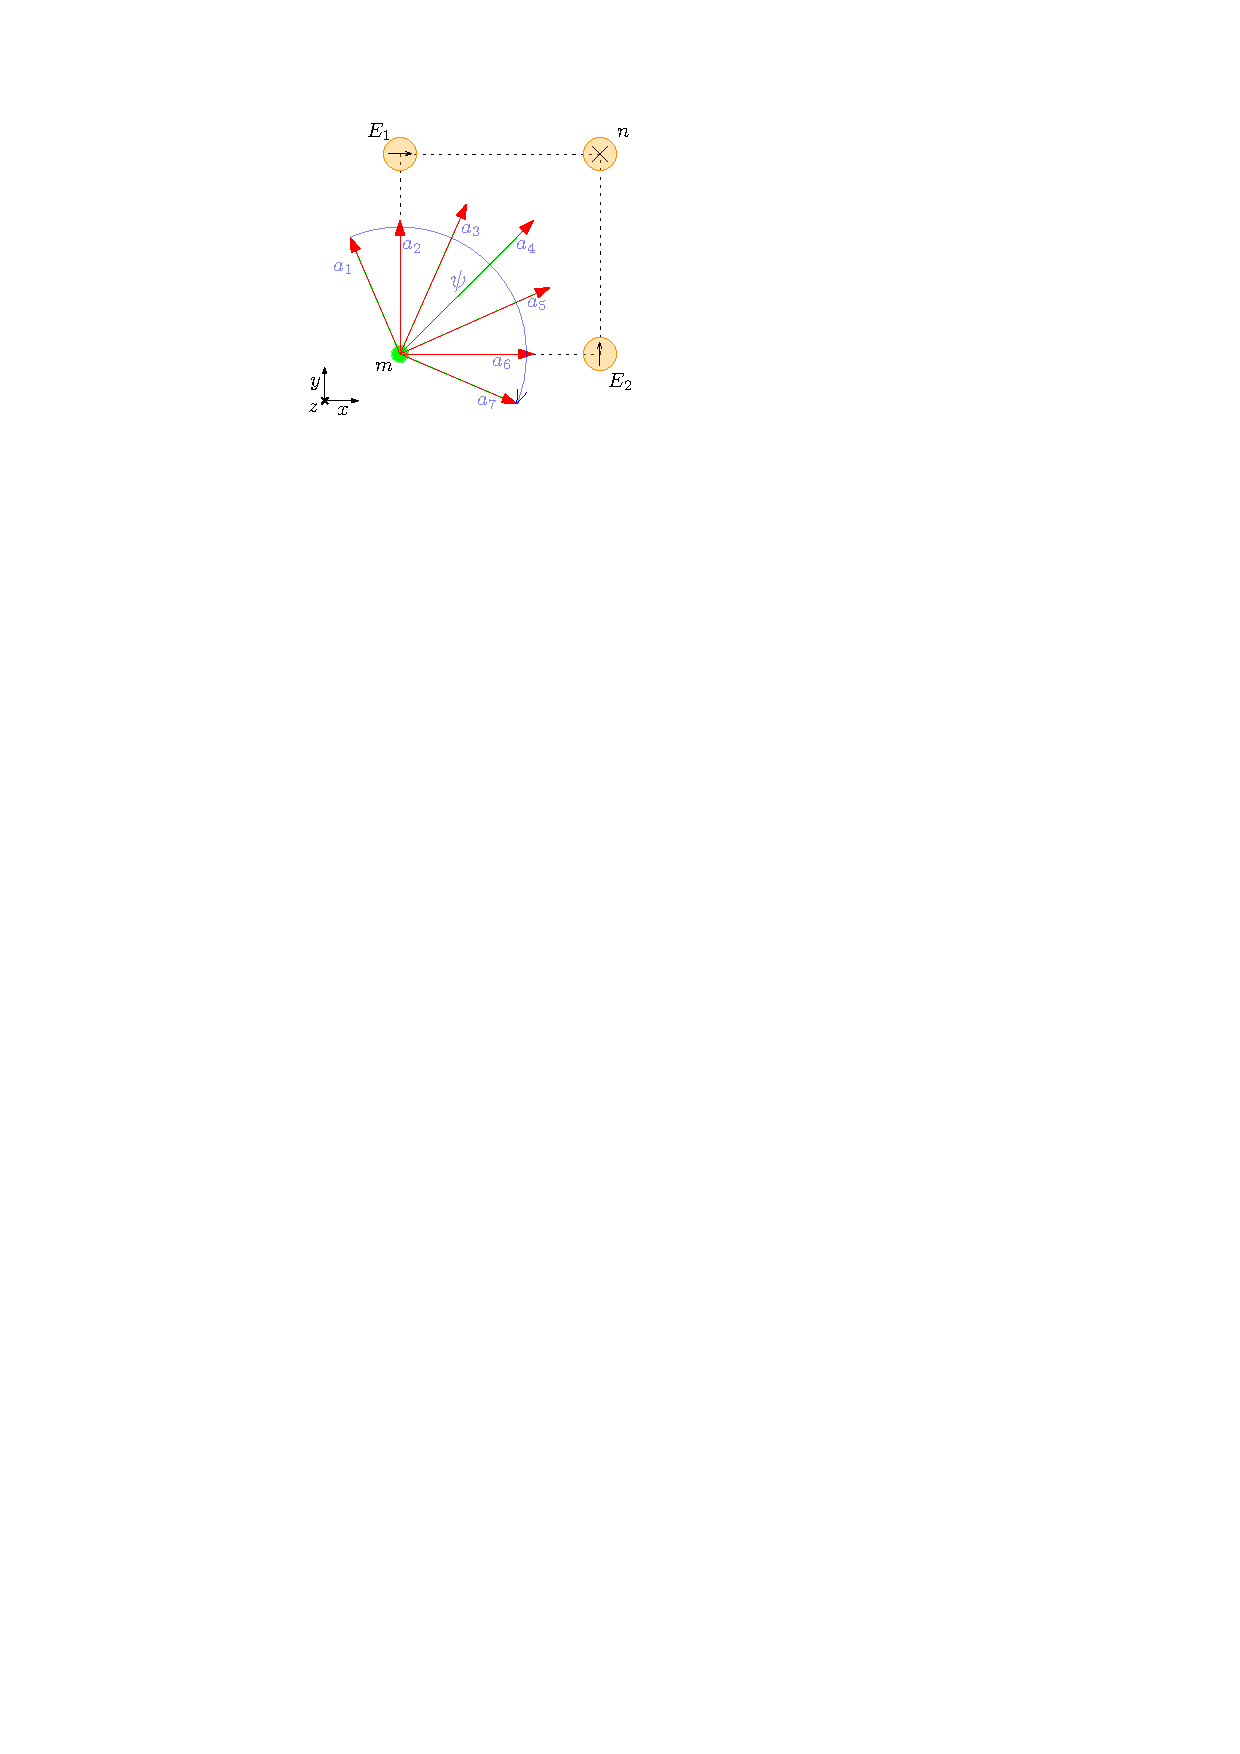
\includegraphics{figures/nonconvexity_of_loss.pdf}
    \caption{Sketch depicting the architecture used in the proof of Lemma \ref{lemma:nonconvexity_loss}. The red arrow depict the various angles $\psi$ of the direction of $m.vel$.}
    \label{fig:nonconvexity_loss}
\end{figure}

\begin{figure}
    \centering
    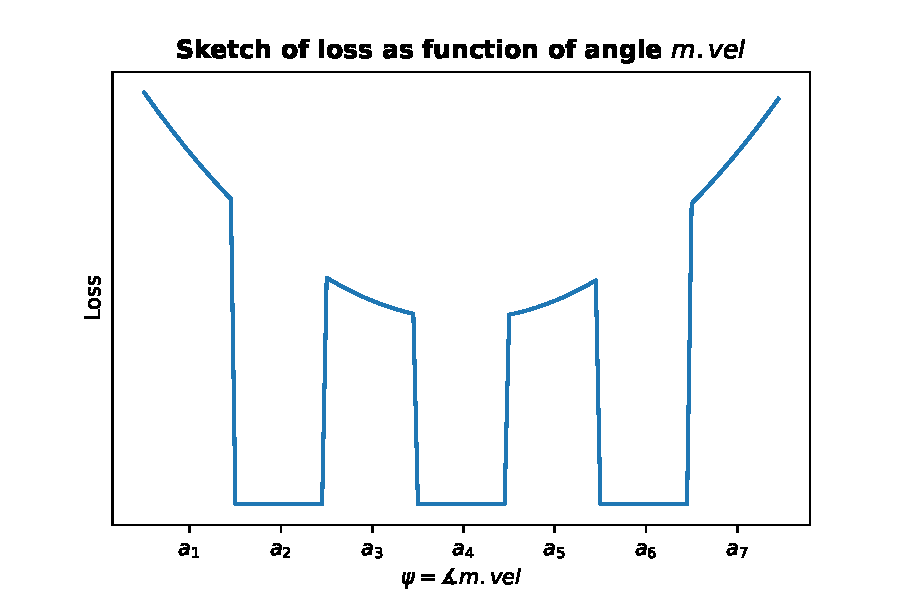
\includegraphics{plot_nonconvex_loss.pdf}
    \caption{Sketch depicting loss function $L(\hat{\vec{y}}, \vec{y})$ as a function of the angle $\psi$ of $m.vel$, in the architecture used in the proof of Lemma \ref{lemma:nonconvexity_loss}.}
    \label{fig:nonconvexity_loss_plot}
\end{figure}

\clearpage

\subsubsection{Loss gradient}

Let $p$ and $s$ be particles, then define the $stiffness$ function as:
\begin{equation}
    stiffness(p, s) = 
    \begin{cases}
        p.\texttt{marble\_stiffness} &\text{if $s$ is a Marble} \\
        p.\texttt{node\_stiffness} &\text{if $s$ is a Node} \\
    \end{cases}
\end{equation}


Using Eq. \eqref{eq:def_pos}, \eqref{eq:def_vel}, \eqref{eq:def_f_net} and \eqref{eq:def_acc} to describe the state of some particle $p$ at a point in time $t=t_1$, we can rewrite the state as follows (assuming that the amount of particles in the architecture is finite):
\begin{align}
    p.pos(t = t_1)  &= p.pos(t = t_1 - 0) + 0 
                    = \lim_{\varepsilon \downarrow 0}\Big(p.pos(t = t_1 - \varepsilon) + p.vel(t = t_1 - \varepsilon) \cdot \varepsilon \Big) \label{eq:pos_eps}\\
    p.vel(t = t_1)  &= p.vel(t = t_1 - 0) + 0 
                    = \lim_{\varepsilon \downarrow 0}\Big(p.vel(t = t_1 - \varepsilon) + p.acc(t = t_1 - \varepsilon) \cdot \varepsilon \Big) \label{eq:vel_eps} \\
    p.acc(t = t_1)  &= \smashoperator{\sum_{\substack{\text{particles $s$}\\\text{ acting on $p$}}}}stiffness(p, s)\cdot\frac{p.mass \cdot s.mass}{p.pos(t=t_1 + 0)-s.pos(t=t_1 + 0)} \nonumber \\
    &= \lim_{\varepsilon \downarrow 0}\Big(\smashoperator{\sum_{\substack{\text{particles $s$}\\\text{ acting on $p$}}}}stiffness(p, s)\cdot\frac{p.mass \cdot s.mass}{p.pos(t=t_1 -\varepsilon)-s.pos(t=t_1 -\varepsilon)}\Big) \label{eq:acc_eps}
\end{align}

Limits cannot be numerically represented on a digital computer. However, we can use a small finite-valued $\varepsilon > 0$, $\varepsilon \in \mathbb{R}$, and then it \textit{approximately} holds that:
\begin{align}
    p.pos(t = t_1)  &= p.pos(t = t_1 - 0) + 0 
                    \approx p.pos(t = t_1 - \varepsilon) + p.vel(t = t_1 - \varepsilon) \cdot \varepsilon \label{eq:pos_eps_approx}\\
    p.vel(t = t_1)  &= p.vel(t = t_1 - 0) + 0 
                    \approx p.vel(t = t_1 - \varepsilon) + p.acc(t = t_1 - \varepsilon) \cdot \varepsilon \label{eq:vel_eps_approx} \\
    p.acc(t = t_1)  &\approx \smashoperator{\sum_{\substack{\text{particles $s$}\\\text{ acting on $p$}}}}stiffness(p, s)\cdot\frac{p.mass \cdot s.mass}{p.pos(t=t_1 -\varepsilon)-s.pos(t=t_1 -\varepsilon)} \label{eq:acc_eps_approx}
\end{align}

Furthermore, note that for some $t_1 > t_0$, where $t_0$ is the starting time (at which each initially existing particle has its original position and velocity):
\begin{align}
    p.pos_0 &= p.pos(t=0) = p.pos(t = t_1 - t_1) \approx p.pos(t = t_1 - \varepsilon \varrho t_1) \label{eq:end_of_recursion}
\end{align}
for some positive constant $0 < \varrho < 1$ defined such that $\varrho t_1 \in \mathbb{Z}$.

We can use the above approximations to rewrite the position of a particle $p$ as a recursive function though time depending on earlier states:

\begin{align}
    p.pos(t = t_1)  &= p.pos(t = t_1 - 0) + 0 
                    \approx p.pos(t_1 - \varepsilon) + \varepsilon \cdot p.vel(t_1 - \varepsilon) \nonumber \\
                    &\approx p.pos(t_1 - \varepsilon) + \varepsilon \Big(  p.vel(t_1 - 2\varepsilon) + \varepsilon \cdot p.acc(t_1 - 2\varepsilon) \Big)\nonumber \\
                    &\approx p.pos(t_1 - \varepsilon) + \varepsilon \Big(  p.vel(t_1 - 2\varepsilon) \nonumber \\ &+ \varepsilon \cdot \smashoperator{\sum_{\substack{\text{particles $s$}\\\text{ acting on $p$}}}}stiffness(p, s)\cdot\frac{p.mass \cdot s.mass}{p.pos(t=t_1 -3\varepsilon)-s.pos(t=t_1 -3\varepsilon)} \Big) \label{eq:pos_recursive}
\end{align}
The terms $p.pos(t=t_1 - 2\varepsilon)$ and $p.vel(t = t_1 - 2\varepsilon)$ can again be expanded using \eqref{eq:pos_eps_approx} and \eqref{eq:vel_eps_approx}. Assume that no MarbleEmitterNodes are present and no inputs are given. Consider the scenario where one continues this process, and applies \eqref{eq:end_of_recursion} where this approximation is reasonable. If no circular recursion occurs (i.e. the sequence of substitutions does not produce a term that was previously substituted), then eventually an expression will be obtained in only the variables $k.mass$ and $k.pos_0$ for all particles $k$ in the architecture. These variables are adjustable parameters, and the applied operations are division, multiplication and subtraction. Hence is the desired output time and location are known, then the Backpropagation algorithm can be applied, in combination with, for example, Gradient Decent, to optimize the architecture.

Now let $m$ be an input that is given to the architecture at some time $t_{input} > t_0$. Let $m.pos_0 = m.pos(t_{input})$. Using Eq. \eqref{eq:pos_eps_approx}, \eqref{eq:vel_eps_approx} and \eqref{eq:acc_eps_approx}, which are all differentiable, we can recursively compute $\frac{\partial L}{\partial m.pos_0}$. Now recall that a \nenwin instance is defined with a function that maps external data to input Marbles (the \texttt{placement\_funct} argument in the pseudocode Algorithm \ref{alg:Nenwin_V1}). If this function has learnable parameters, then $\frac{\partial L}{\partial m.pos_0}$ depends on those, and hence Backpropagation can optimize the function's parameters via $\frac{\partial L}{\partial m.pos_0}$.

\subsection{Backpropagation of mass-gradient through MarbleEmitterNodes}
Now consider a Marble $m$ that is produced by a MarbleEmitterNode $n$. Let $n.spawnpos$ be the relative position of $m$ with respect to $n$ when $m$ was emitted, and $m.pos_0$ be the absolute position where $m$ was spawned. Now $m.spawnpos$ and $m.mass$ are parameters of $n$, and $n$ is initially present in the architecture. 
A difficulty arises, since $m.pos_0$ depends on the time $t = \hat{t}_0$ at which $m$ was created, which depends on on the \texttt{stored\_mass} of $n$. 
$n.stored\_mass$ can be seen a non-smooth function of time and the set of consumed Marbles
(which in turn depend on their initial position, attraction by other particles, their mass, etc.):
\begin{equation}
    n.stored\_mass(t) = \qquad \smashoperator{\sum_{k \in n.eaten\_marbles}} k.mass \qquad - \qquad \smashoperator{\sum_{h \in emitted\_marbles(n)}} h.mass \geq 0
\end{equation}
Where $emitted\_marbles(n)$ denotes the set of Marbles previously emitted by $n$. 
This set only exist conceptually: no variable or attribute has been defined to track it.


One way to resolve this issue is to see the \texttt{stored\_mass} 
together with the mass of the stored Marbles and the emitted mass as one continuum. 
In this case, $m.pos_0$ only depends on the last $x$ consumed Marbles by $n$ at $t = \hat{t}_0$ that together have sufficient mass, i.e.
\begin{equation}
    x = \min_{\hat{x} \in \mathbb{Z}} (\hat{x} : \left(\sum_{i = \hat{x}}^{\norm{n.eaten\_marbles(\hat{t}_0)}} n.eaten\_marbles(\hat{t}_0)[i].mass\right) \geq m.mass )
\end{equation}
where we use the fact that $n.eaten\_marbles$ is a stack with references to the Marbles consumed by $n$. For convenience, call this set of $x$ Marbles $X$.

Now between being consumed and being emitted, the quantity of mass that is $m.mass$ is 'frozen': it does not take part in any multiplication (except for the comparison whether $m$ can already be emitted). Hence, under the assumption that $m.mass$ directly depends on the mass of the last $x$ consumed Marbles (before $m$ was emitted), and that inclusion in this set $X$ directly depends on the \textit{last} position of each Marble in $X$. It will be assumed that these direct dependencies can be modelled with a derivative of 1, i.e. for all $m_i \in X$ that are consumed by $n$ at time $t_i$:
\begin{align}
    \frac{\partial m.pos_0}{\partial m_i.mass} = 1 \label{eq:deriv_emitted_to_mass}\\
    \frac{\partial m.pos_0}{\partial m_i.pos(t_i)} = 1 \label{eq:deriv_emitted_to_pos}
\end{align}
Eq. \eqref{eq:deriv_emitted_to_mass} and \eqref{eq:deriv_emitted_to_pos} are the 'missing link' that allows Backpropagation though MarbleEmitterNodes. Note that strong assumptions have been made, that need to be justified by experimental results\footnote{This will remain a topic for further research, as a better approach might be desirable.}. 
A disadvantage of this approach is that $n.radius$ is considered to be fixed, and cannot be optimized.

% The derivatives of $m.pos_0$ with respect to the other parameters of the MarbleEmitterNode itself can directly be computed, using the definition of $m.pos_0$: 
% \begin{align}
%     m.pos_0 = n.spawnpos + n.pos(t = \hat{t}_0) \\
%     \frac{\partial m.pos_0}{n.spawnpos} = 1 \\
%     \frac{\partial m.pos_0}{n.pos(\hat{t}_0)} = 1
% \end{align}

\subsection{Backpropagation of pos-, vel- and acc-gradient through MarbleEmitterNodes}
The above description allows to find the gradient of the mass of an emitted Marble $m$ with respect to the Marbles consumed by the MarbleEmitterNode $n$, and $n$ itself. But also the gradient of the loss with respect to the initial position of the Marble can be used to optimize $n$. Note that $m$ is created when certain variables (the time passed since last emit and $\norm{n.stored\_mass}$) exceed a certain threshold ($n.delay$ and $\norm{m.mass}$). 
\begin{align}
    m.pos_0 &= n.pos(t) + n.spawnpos \\
    \frac{\partial m.pos_0}{\partial n.pos(t)} &= \vec{1} \\
    \frac{\partial m.pos_0}{\partial n.spawnpos} &= \vec{1}
\end{align}

\subsection{Non-propagatable gradients}

The position and the mass are special cases where the gradient of a loss with respect to a variable of the emitted Marble can be propagated back to the MarbleEmitterNode and the particles that influenced the MarbleEmitterNode. For other variables of the Marble, such as the initial velocity and acceleration, this does not seem to be the case. The acceleration is a function of the particles that are present in the neighbourhood of the place where the Marble is created, hence it is intuitive that this is not differentiable to the MarbleEmitterNode. For the velocity (and any other ordinary variable that extensions of Marbles may have) this might less intuitive.

It can be shown by using a general case. Consider an object with variable $v$ is created at a certain point in time $\hat{t} > 0$ where some time-varying variable $x(t)$ meets a certain threshold $\theta$. Then initial value of $v$ at $\hat{t}$, $v_0$, can be written as a function of $\theta$ and $x$. Let $\hat{v}$ be the predefined value that becomes \textit{assigned} to $v$ at $t = \hat{t}$. Note that \textit{the value of} $v_0$ is independent of the value of $x(t)$ and vice-versa ($v_0$ is only created when $x(t) \geq \theta$, hence we always have $ReLU(\text{sgn}(\norm{x(\hat{t}) - \theta})) = 1$ when $v_0$ is created).

We have 
\begin{align}
    v_0 &= v_0(x(t), \theta) = \hat{v} \cdot ReLU(\sgn(\norm{x(\hat{t}) - \theta})) \\
    \frac{\partial v_0}{\partial x} &= \hat{v} \cdot \frac{\partial ReLU}{\partial \text{sgn}} \cdot \frac{\partial \text{sgn}}{\partial x} \\
    \frac{\partial v_0}{\partial \theta} &= \hat{v} \cdot \frac{\partial ReLU}{\partial \text{sgn}} \cdot \frac{\partial \text{sgn}}{\partial \theta}
\end{align}
\hl{Add arguments to ReLU and sgn!}

%\subsubsection{Backpropagation with inputs}
% \hl{
% Hence Eq. \eqref{eq:end_of_recursion} still applies, only with a different value of $\varrho$ than for particles that are initially already present in the architecture. However, the moment in time at which $m$ is created also depends on the Marbles $n$ has consumed earlier. For a correct optimization, Backpropagation needs to propagate though these Marbles as well.

% Let $\frac{\partial L}{\partial m.pos_0}$ be the gradient of the computed loss function with respect to the position where $m$ was 'spawned' at the time $t = \hat{t}_0$ when $m$ was created. Any Marble $k$ that had not been consumed by $n$ at time $t = \hat{t}_0$ had no direct influence on the creation 

% Also for input Marbles 
% }

\subsection{Backpropagation discussion}
The training theory described above can only be applied if an output has been received. If no output is provided by the architecture, then it is ambiguous which Marble was required to be consumed by a specific MarbleEaterNode at a specific point in time. To resolve this, it is possible to assign a particular Marble a priori to be the output, or design the architecture in such a way that an output will always be given after sufficient time.

It is worth stressing that no known convex loss function exists for this optimization, so Gradient Descent might in general fail to find a global optimum. However, the attained local optima might still be of sufficient quality for the method to be of practical value. Further below, experimental performance will be discussed.


An alternative view on the reasoning above is that \eqref{eq:pos_eps_approx}, \eqref{eq:vel_eps_approx} and \eqref{eq:acc_eps_approx} are a numerical integration of a system of differential equations. Following this line of thought, also other explicit integration methods can be used for training. Since a numerical integration is needed in implementation to simulate the dynamics in Nenwin, this can effectively be combined with the training of the architecture.
    
    \section{Experimental results}
    The classification scheme as described above has been used on the Banknote Authentication dataset \cite{banknote_paper} (downloaded from \cite{banknote_download}\footnote{Note that this page explains the labels the wrong way around. See \cite{genuine_class_banknote}}).
This particular dataset was chosen because it required only few particles to encode the input and the output:
\begin{enumerate}
	\item There are only two distinct labels (binary classification).
	\item Each input vector contains only four elements.
\end{enumerate}

The implementation is available at \url{https://github.com/Nifrec/nenwin} under the open-source AGPL-3.0 licence\cite{AGPL_3}.

Note that these experiments are intended to give an indication of trainability and parameter sensitivity of the \textsc{Nenwin} framework. 
A full search-space evaluation is beyond the scope of this report (and would require a more optimized implementation).

\subsection{Dataset description}
The classification task is to classify banknotes as genuine or as forgeries, 
given four derived features from the images. 
Class 0 has 762 samples and represent the genuine banknotes,
class 1 has 610 represents the forgeries. 
This split is close to a 50\%/50\% split, meaning that random classification would yield an accuracy around 50\%.
The derived features (of Wavelet-transformed image) have been pre-computed, and are:
\begin{enumerate}
	\item Variance
	\item Skewness
	\item Kurtosis
	\item Entropy
\end{enumerate}

For the experiments, the samples of the dataset were shuffled in a random order and split in a 80\%/10\%/10\% train/validation/test set split. This split was cached and reused for each experiment (i.e. each experiment had the same train, validation and test set).

\subsection{Architectures}
Three different architectures have been designed and were evaluated. See also Fig. \ref{fig:banknote_architectures}.

\paragraph{Architecture A:}
\begin{itemize}
	\item Vertices of input region: (-2.5, -1), (-2.5, 1), (2.5, -1), (2.5, 1).
	\item 4 non-output nodes surrounding the input region (positions (0, -5), (-5, 0), (5, 0) and (0, 5)).
	\item MarbleEaterNodes (output Nodes) at (-10, 0) and (10, 0).
\end{itemize}

\paragraph{Architecture B:}
Same as Architecture A, but with additional Nodes at (2.5, 2.5), (-2.5, 2.5), (2.5, -2.5), (-2.5, -2.5).

\paragraph{Architecture C:}
\begin{itemize}
	\item Vertices of input region: (0, 0), (0, 1), (6, 0), (6, 1).
	\item 5 non-output nodes surrounding the input region (positions (1, 2), (2, 3), (3, 2), (4, 3) and (5, 2)).
	\item MarbleEaterNodes (output Nodes) at (1, 4) and (5, 4).
\end{itemize}

\begin{figure}
	\centering
	\begin{subfigure}[b]{0.3\textwidth}
		\centering
		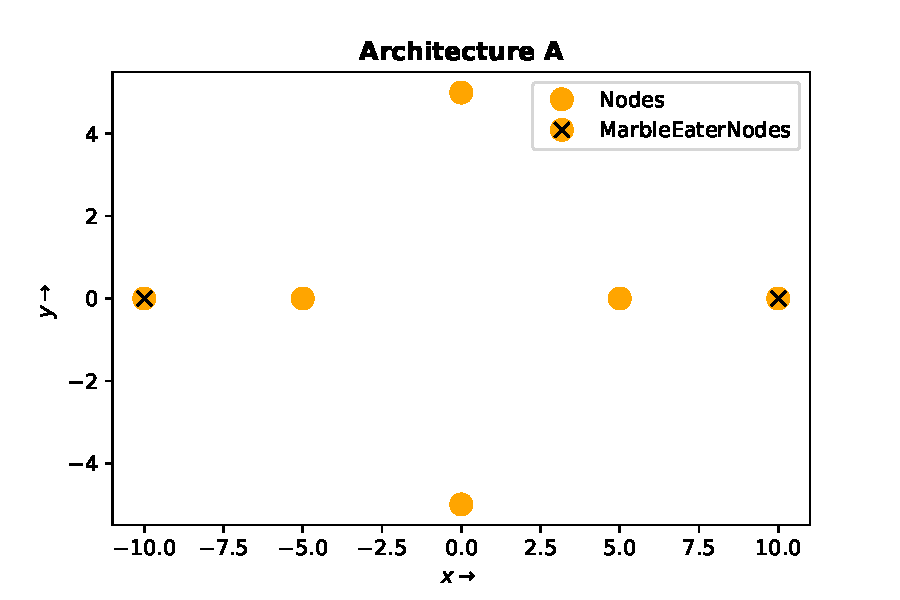
\includegraphics[width=\textwidth]{figures/architecture_A.pdf}
		\label{fig:architecture_a}
	\end{subfigure}
	\begin{subfigure}[b]{0.3\textwidth}
		\centering
		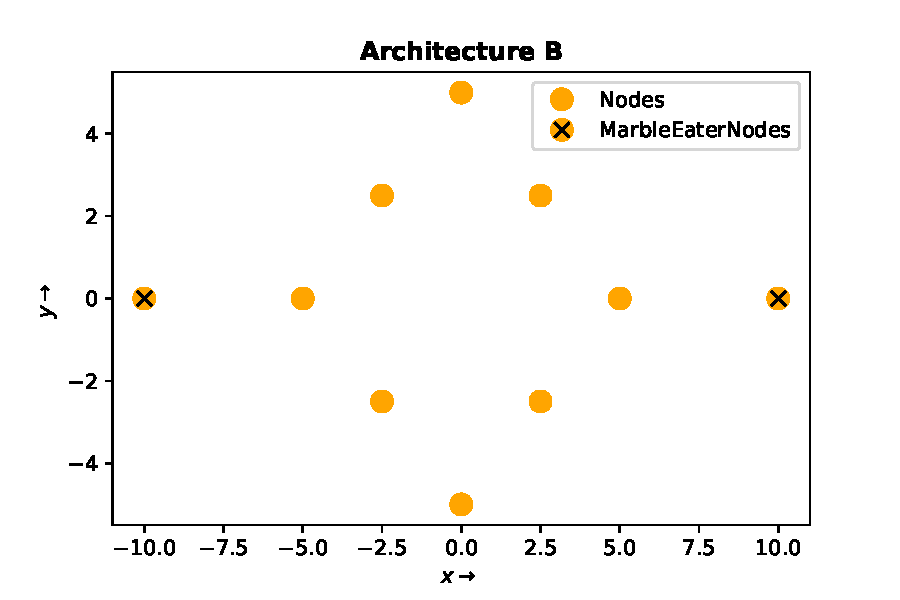
\includegraphics[width=\textwidth]{figures/architecture_B.pdf}
		\label{fig:architecture_b}
	\end{subfigure}
	\begin{subfigure}[b]{0.3\textwidth}
		\centering
		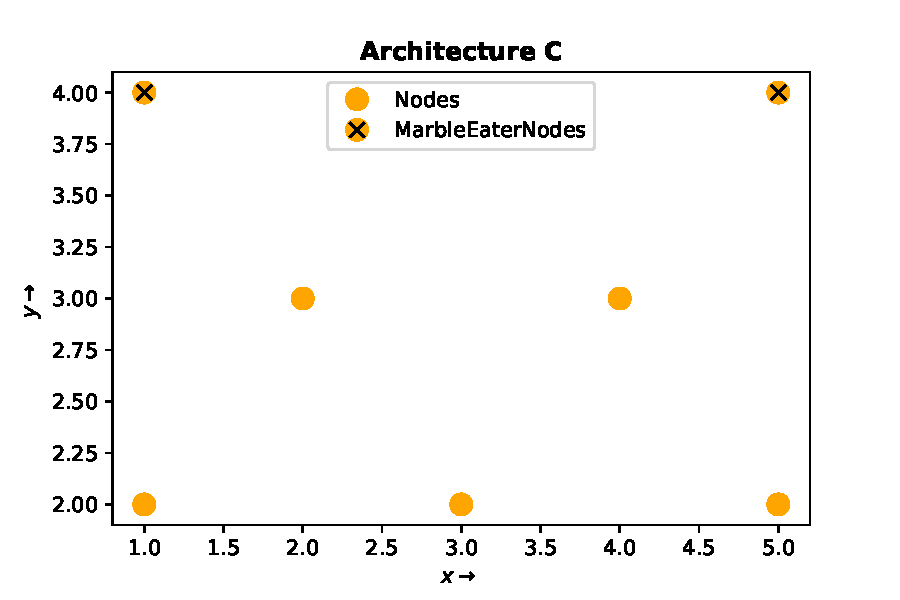
\includegraphics[width=\textwidth]{figures/architecture_C.pdf}
		\label{fig:architecture_c}
	\end{subfigure}

	\caption{\textsc{Nenwin} Architectures used for training on the banknote dataset.}
	\label{fig:banknote_architectures}
\end{figure}

\subsection{Setup}
For each experiment, one of the architectures A, B or C was generated, and other hyperparameters were chosen.
In particular, the batch size and the input placer were varied. 

The training procedure used was as follows:
during each epoch, the samples of the training set are iterated in a random order. 
Each sample in the training set converted to Marbles by the chosen input placer.
Then the simulation is run until at least one MarbleEaterNode ate a Marble, 
or until a maximum number of steps is reached. 
Then the loss is computed according to \eqref{eq:classification_loss_full},
and gradients of parameters with respect to this loss are computed via backpropagation.
Finally the parameters are updated using the Adam optimization technique.

The average gradient is used in case the batch size is larger than 1. 
The samples are still processed in sequential order, but the gradients of their losses are accumulated.
The Adam update rule is only used after the last sample in the batch.

Because of practical resource and time constraints, this maximum amount of timesteps was set to only 20 steps, with a stepsize of 0.1. 
With this configuration it took several hours to train an architecture\footnote{Training was run on a a Intel(R) Core(TM) i7-7700HQ CPU @ 2.80GHz.}. 

\subsection{Results}

Numerical results of various training-runs have been summarized in Table \ref{table:banknote_exp}. 

\begin{table}[hb]
	\begin{tabular}{lll|lll}
		\textbf{Architecture} &
		\textbf{Timesteps} &
		\textbf{\begin{tabular}[c]{@{}l@{}}input\\ placer\end{tabular}} &
		\textbf{\begin{tabular}[c]{@{}l@{}}batch\\ size\end{tabular}} &
		\textbf{\begin{tabular}[c]{@{}l@{}}validation\\ accuracy\end{tabular}} &
		\textbf{\begin{tabular}[c]{@{}l@{}}training\\ loss\end{tabular}} \\ \hline
		A & 20 & VelInputPlacer  & 1 & 0.17518 & 20307.7 \\
		A & 20 & VelInputPlacer  & 2 & 0.13869 & 21173.4 \\
		A & 20 & VelInputPlacer  & 5 & 0.06569 & 28580.8 \\
		A & 20 & MassInputPlacer & 1 & 0.0     & 13.5    \\
		C & 20 & MassInputPlacer($\begin{bmatrix} 1\\1\end{bmatrix}$) & 1 & 0.0 & 200.1 \\
		B & 20 & VelInputPlacer  & 2 & 0.12409 & 24788.9 \\
		C & 20 & VelInputPlacer  & 2 & 0.08029 & 33143.6 \\
		C & 36 & MassInputPlacer($\begin{bmatrix} 0.5\\0\end{bmatrix}$) & 1 & \textbf{0.51825} & -1198.1 \\
		C & 40 & MassInputPlacer($\begin{bmatrix} 0.5\\0\end{bmatrix}$) & 1 & 0.20438 & -4590.7
	\end{tabular}
	\caption{Results of training a \nenwin architecture on the banknote-authentication dataset. Each row represents an independent training run. The accuracy is the total amount of correct predictions divided over the size of the validation set. Absence of output is counted as a wrong prediction. The loss accumulation of losses of the last epoch of the train set.}
	\label{table:banknote_exp}
\end{table}

Using the VelInputPlacer appears to providing poor results. A plot of the performance per epoch shows that the training initially makes progress, but converge too quickly to mediocre performance. See Fig. \ref{fig:velinputplacer_performance}. One possible explanation is that the VelInputPlacer gives the input Marbles a high initial velocity in varying directions. With a very limited amount of Nodes the model may not posses the flexibility handle all combinations of initial velocity directions of the Marbles. 

\begin{figure}[hb]
	\centering
	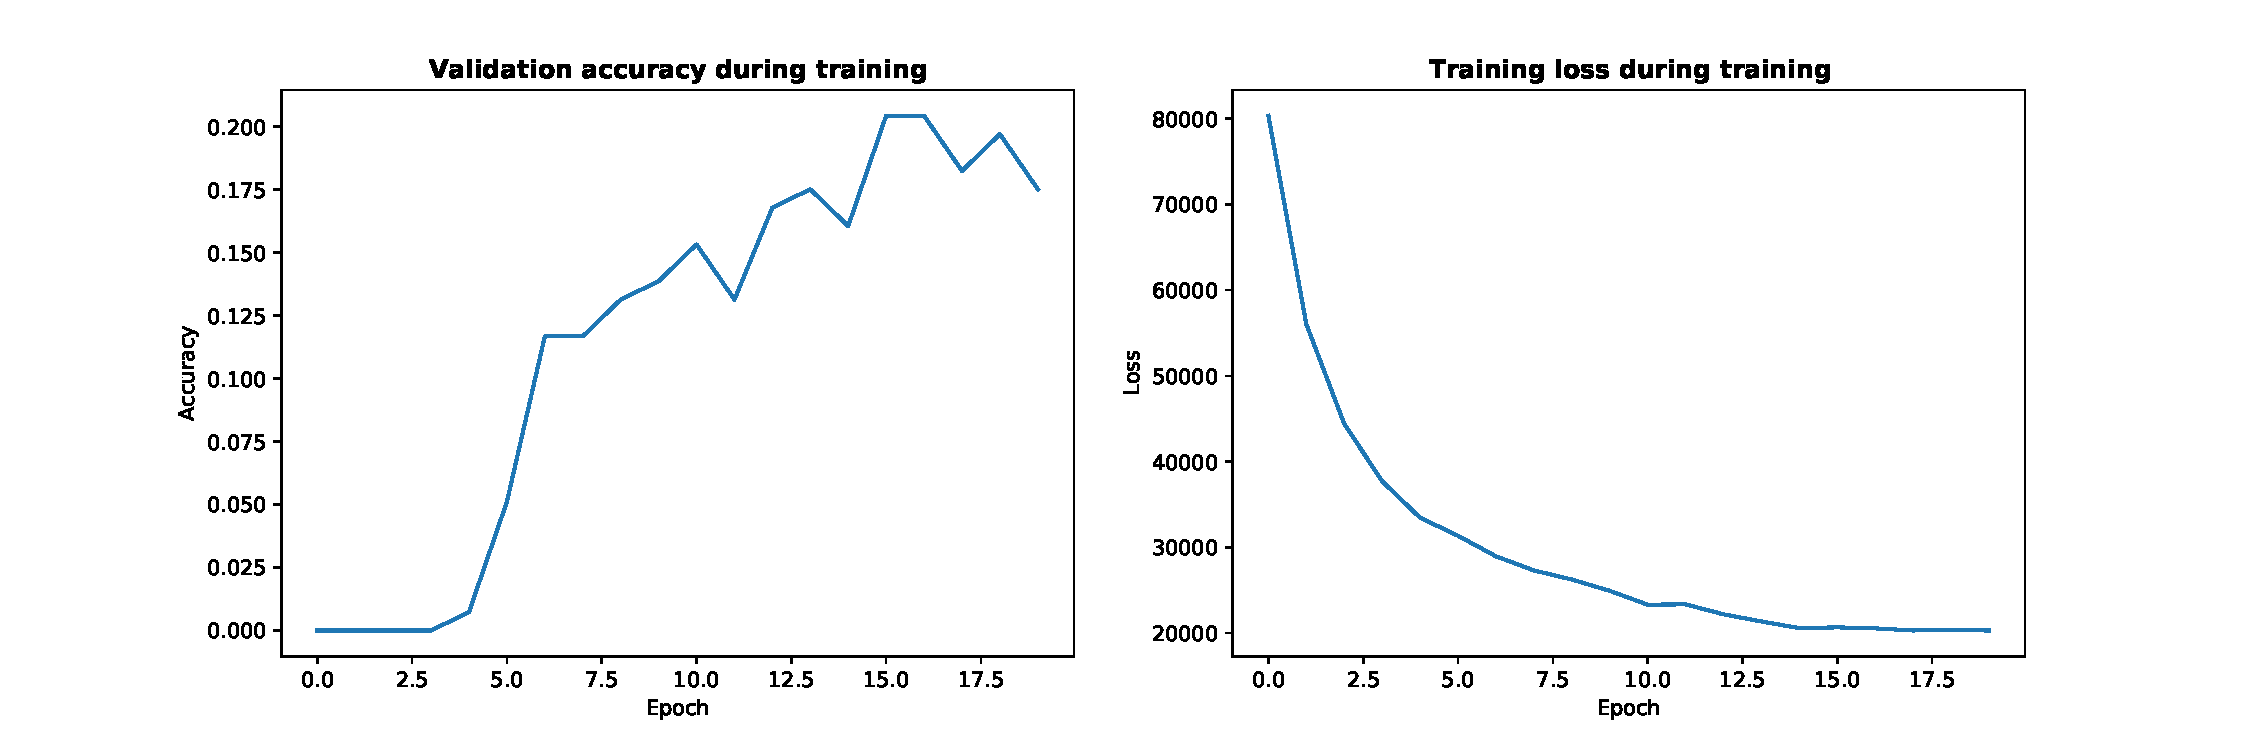
\includegraphics[scale=0.4]{figures/A_batch1_velinputplacer.pdf}
	\caption{Performance of Architecture A as measured during each epoch of training. The VelInputPlacer was used to map the four banknote features to four Marbles. The batch size was 1. Note how the improvement of the accuracy on the validation set already seems to destabilize and cease rapid growth in less than 20 epochs. Given that the decrease in train set loss also flattened out at this time, it would seem unlikely that running more epochs would significantly increase the validation set accuracy.}
	\label{fig:velinputplacer_performance}
\end{figure}

\clearpage

The most surprising results are obtained with the MassInputPlacer with a velocity vector of $\begin{bmatrix} 0.5\\0\end{bmatrix}$ starting with Architecture C. Note that Marbles will be moving towards the MarbleEaterNodes with this initial velocity in Architecture C. After 36 epochs this resulted in a validation-set accuracy above chance level, see Fig. \ref{fig:arch_c_const_vel_50pc_learning_curve}. However, the learning curve shows very eccentric patterns. The high validation set accuracy after 36 epochs quickly disappeared after more epochs. This might be due to overfitting, although it is a very sudden change. The high non-convexity of the training objective may be a more likely explanation. One hypothesis is that the optimization rule might have stepped a bit too far in a certain direction (by updating the parameters), and entered the domain of the loss function which has a different local minimum. This is for example possible if the optimization step caused a small adjustment that made a Marble being eaten early in the simulation, which would otherwise bypass the MarbleEaterNode. This would change the moment that the loss in computed. This may result in a very different loss, as the other Marbles will be at very different positions than at the end of the maximum simulation time.

The train-set loss also shows an extreme outlier, which occurs at the first epoch in the accuracy on the validation set experienced a sudden increase. 

Also see Fig. \ref{fig:arch_c_const_vel_50pc_architecture} for a comparison of Architecture C before and after 40 epochs of training. The architecture changed significantly. The output Nodes have been moved towards the input region.

\begin{figure}[hb]
	\centering
	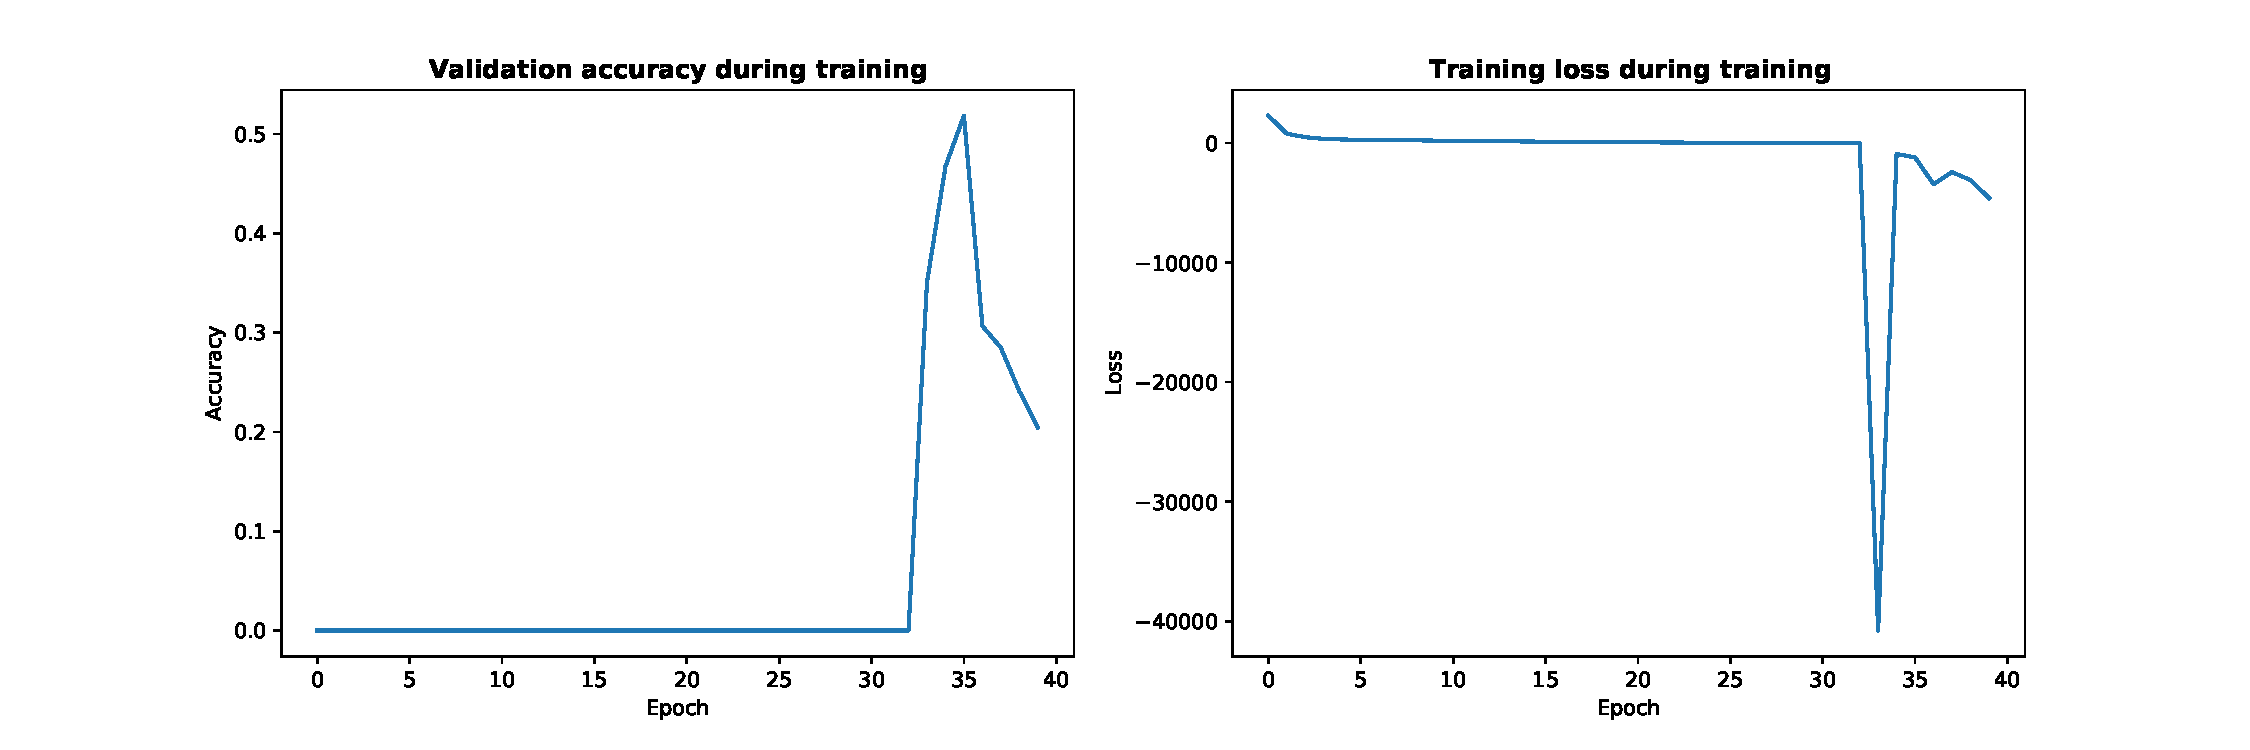
\includegraphics[scale=0.4]{figures/C_batch1_ConstVelInputPlacer([0.5, 0]])_epoch40_stats.pdf}
	\caption{Learning curves of using Architecture C with 
		a batch size of 2, MassInputPlacer($\begin{bmatrix} 0.5\\0\end{bmatrix}$) and 40 train-set epochs.}
	\label{fig:arch_c_const_vel_50pc_learning_curve}
\end{figure}

\begin{figure}[hb]
	\centering
	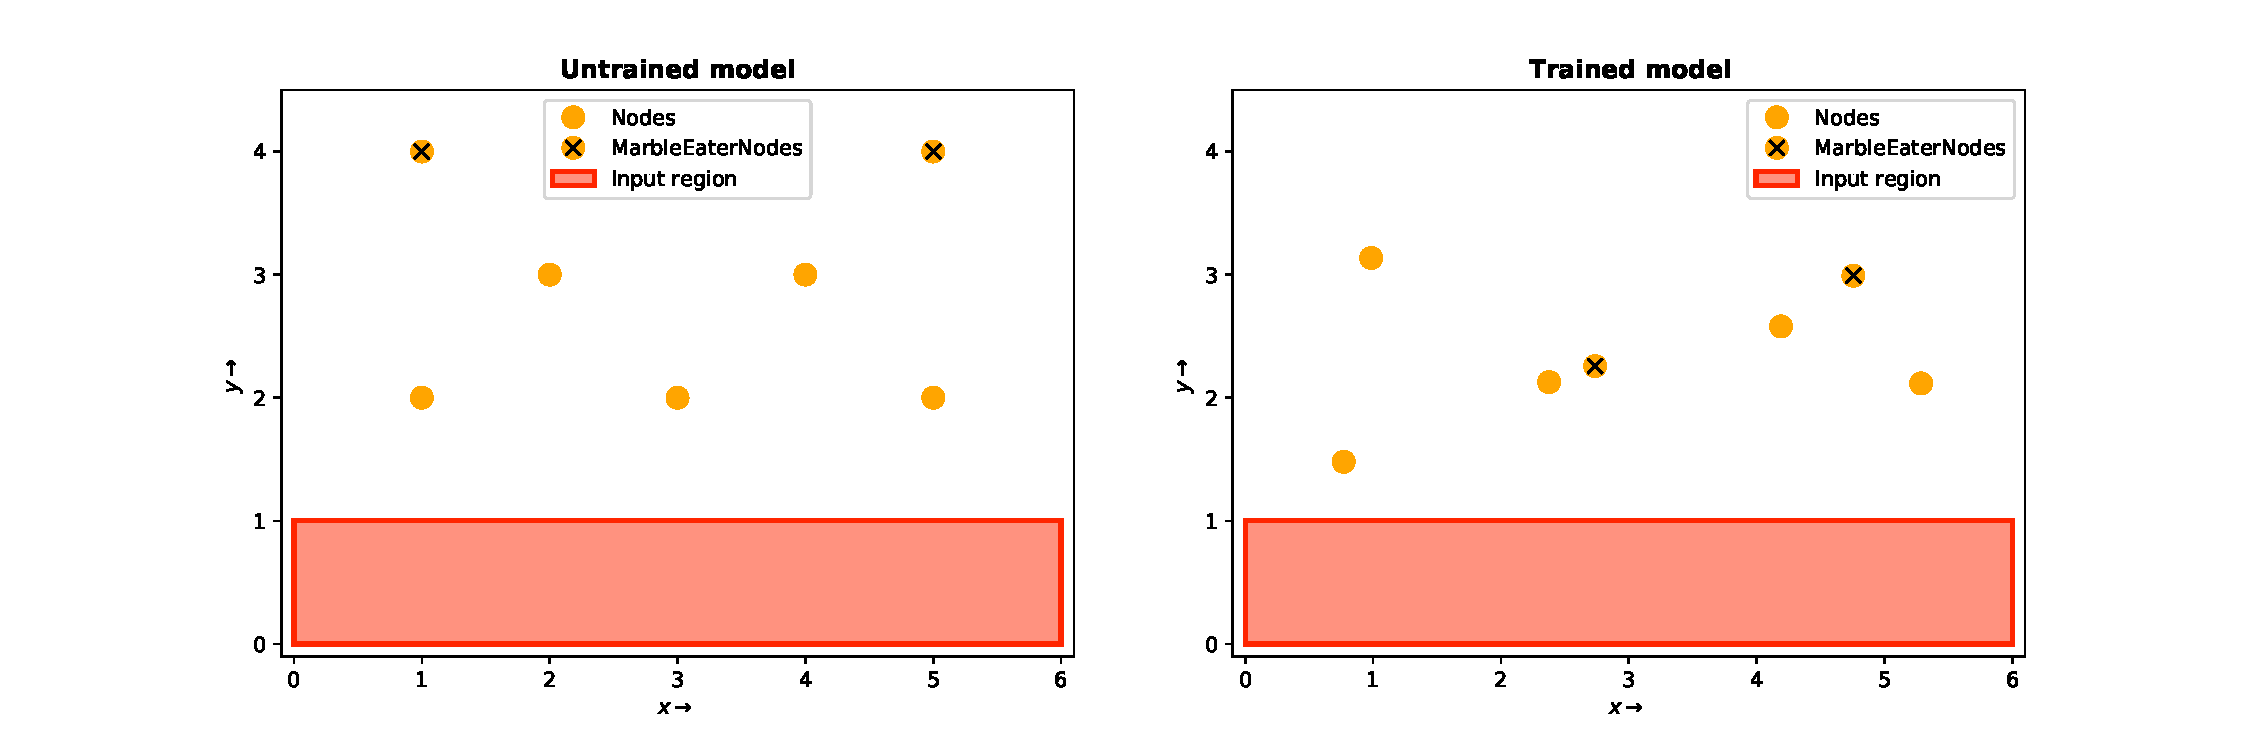
\includegraphics[scale=0.4]{figures/C_batch1_ConstVelInputPlacer([0.5, 0]])_epoch40.pdf}
	\caption{Architecture C before training (left) and after training on 40 epochs with 
		a batch size of 2, MassInputPlacer($\begin{bmatrix} 0.5\\0\end{bmatrix}$).}
	\label{fig:arch_c_const_vel_50pc_architecture}
\end{figure}

\clearpage
    
    \section{Complexity}
    This section will explore the runtime and memory complexity of the simulation of \textsc{Nenwin}. \textsc{Nenwin} itself is specified as a continuous system, mainly governed by Eq. \eqref{eq:def_pos}-\eqref{eq:def_acc}. These differential equations cannot be analytically computed, so a discrete numerical integration approximation is used. With a specific integration algorithm in place, it is possible to derive the runtime complexity and the memory needs for backpropagation.

\subsection{Beeman' s Algorithm}
Our implementation uses a variant of Beeman's Algorithm to numerically integrate Eq. \eqref{eq:def_pos}-\eqref{eq:def_acc}. Beeman's Algorithm was first published by Schofield in 1972 \cite{beemans_alg}. The variant we used was published by Beeman himself in \cite{BEEMAN1976}, and is a direct integration method. Applied to a particle $p$ in \textsc{Nenwin}, we update the particle' s motion each timestep as follows:

\begin{align}
    p.pos(t) & = p.pos(t-h) + h \cdot p.vel(t-h) + \frac{1}{6} h^2 \cdot (4p.acc(t-h) - p.acc(t-2h)) \label{eq:beeman_pos}\\
    p.vel(t) & = p.vel(t - h) + \frac{1}{12}h \cdot (5 p.acc(t) + 8 p.acc(t-h) - p.acc(t-2h)) \label{eq:beeman_vel}
\end{align}
where $h$ is the step-size and $t$ the timestamp. Note that, at the beginning at timestep $t$, $p.acc(t)$ is computed according to Newton's gravity function (Eq. \eqref{eq:newton_grav_force}).

\subsection{Runtime complexity}
\begin{lemma}[Runtime complexity]
Assume a $\mathcal{O}(1)$ discrete numerical integration algorithm is used to compute a discrete approximation of \eqref{eq:def_pos}-\eqref{eq:def_acc} for a particle. Let $m$ be a \textsc{Nenwin} architecture. Let $T$ be the number of discrete timesteps the \textsc{Nenwin} algorithm is run on $m$. Let $n$ be the number of particles in $m$. Then the number of operations needed to run the algorithm for $t$ timesteps is bounded by $\mathcal{O}(T\cdot n^2)$.\label{lemma:runtime_complexity}
\end{lemma}
\begin{proof}
Refer to Algorithm \ref{alg:Nenwin_V1}. 

Line 1 only copies a reference. Line 2 and 3 each do a constant amount of work for each Node, so are bounded by $\mathcal{O}(n)$
By definition of $T$, line 4 is executed $T$ times. This is a loop with a long body, consisting of the following: 

Line 19 iterates over all $n$ particles. Line 21, within this loop, iterates over all other $n-1$ particles. Lines 20 and 22-25 are all $\mathcal{O}(1)$. Hence the nested loops of lines 19-25 have an $\mathcal{O}(n^2)$ runtime.

The loops of line 26 and 29 iterate over a subset of all particles and all particles respectively, only only execute a constant amount of work within the loop body, and are hence both $\mathcal{O}(n)$. Finally the loop of lines 32-37 iterates over all Marbles and all MarbleEaterNodes, which are at most $\frac{1}{2}n \times {1}{2}n = \mathcal{O}(n^2)$ iterations.

So in total, the loop of line 4 makes $\mathcal{O}(T \cdot n^ 2)$ iterations, which is therefore also the upper bound of the algorithm.
\end{proof}

\subsection{Backpropagation memory complexity}
Backpropagation requires a computational graph to be created during the simulation. This computational graph stores all algebraic operations applied and all constants needed to derive the partical derivates of a loss with respect to all relevant the inputs and parameters of the simulation. This graph has a fixed size for a neural network, but in \textsc{Nenwin} it depends on the amount of simulated timesteps. To keep the theory brief, we will only consider \textsc{Nenwin} architectures without MarbleEaterNodes and MarbleEmitterNodes.

\begin{lemma}[Backpropagation memory complexity]
Assume Beeman's algorithm \cite{beemans_alg} is used to compute a discrete approximation of \eqref{eq:def_pos}-\eqref{eq:def_acc}. Assume that Newtonian gravity \eqref{eq:newton_grav_force} is used as attraction function. Let $m$ be a \textsc{Nenwin} architecture. Let $T$ be the number of discrete timesteps the \textsc{Nenwin} algorithm is run on $m$. Assume no MarbleEmitterNodes or MarbleEaterNodes are present in $m$. Let $n$ be the number of particles in $m$. Let $d$ be amount of dimensions used in $m$ (i.e. the length of the $pos$, $vel$ and $acc$ vectors). 
%  Let $a_v$ be the upper bound on the amount of gradient-tracking vector variables in each particle. Let $a_s$ be a similar upper bound but for scalar variables. 
Then the amount of memory needed to store all algebraic operations and numerical values in a computational graph for backpropagation is $\mathcal{O}(T \cdot n^2 \cdot (a_v \cdot d + a_s))$.
\end{lemma}
\begin{proof}
Only the $pos$, $vel$ and $acc$ variables of a particle change in value. The $mass$ (and optionally also the stiffness and attraction weights) do require gradients for optimization, but do not change value during simulation (only at the optimization step). Hence they are only leaves in the computational graph. By the same reasoning, the \textit{initial} position, velocity and acceleration are leaves in the computational graph.

\eqref{eq:newton_grav_force} uses one multiplication, a division, vector subtraction, a norm and a scalar square. No non-parameter constants are involved, so this requires an $\mathcal{O}(1)$ amount of memory to store the operations.

We proceed by considering the operations done on the $pos$, $vel$ and $acc$ of a single particle $p$ in one discrete timestep (referring to Algorithm \ref{alg:Nenwin_V1}):
\begin{enumerate}
    \item Lines 21-24 compute the net force on a particle. Line 22 uses a subtraction ($\mathcal{O}(1)$), line 23 a division ($\mathcal{O}(1)$) and a norm of a length-$d$ vector ($\mathcal{O}(1)$), and line 24 an addition ($\mathcal{O}(1)$) and Newton's gravity function ($\mathcal{O}(1)$, as shown above). This is done for each of the other $n-1$ particles (line 21), so a total of $\mathcal{O}(n)$ operations need to be stored.
    \item Line 25 is a $\mathcal{O}(1)$ assignment.
    \item Lines 29-30 execute Beeman's algorithm on each of the $n$ particles. Beeman's algorithm require the previous acceleration, the previous position and the previous-previous acceleration to be cached, but these values are needed for backpropagation. This can be seen as follows, the partial derivatives of Eq. \eqref{eq:beeman_pos} are:
    \begin{align}
        \frac{\partial p.pos(t)}{\partial p.pos(t-h)} & = 1 \\
        \frac{\partial p.pos(t)}{\partial p.vel(t-h)} & = h \\
        \frac{\partial p.pos(t)}{\partial p.acc(t-h)} & = \frac{2}{3}h^2 \\
        \frac{\partial p.pos(t)}{\partial p.acc(t-2h)} & = -\frac{1}{6}h^2 \\
    \end{align}
    which are all scalars. The same reasoning holds for the partial derivatives of Eq. \eqref{eq:beeman_vel}. Storing a fixed amount of scalars takes $\mathcal{O}(1)$ memory. Storing the operations itself also takes a $\mathcal{O}(1)$ amount of memory.
    
    The total memory need for caching information for backpropagation for executing Beeman's algorithm on all particles is $\mathcal{O}(n)$ per timestep. 
\end{enumerate}
Since there are $T$ timesteps, the total memory need is bounded by $\mathcal{O}(T \cdot n)$
\end{proof}

The expression $\mathcal{O}(T \cdot n)$ may hide a large constant factor, and in practice it seems it indeed does so. Furthermore, for advanced applications many particles and many timesteps may be needed. Especially for numerical accuracy a large number of timesteps is desirable. Hence, despite the polynomial complexity, this can easily lead to a high memory cost.
    
    \section{Runtime complexity optimization}
    As shown above (Lemma \ref{lemma:runtime_complexity}), the runtime complexity of a single step of \textsc{Nenwin} is bounded by $\mathcal{O}(n^ 2)$. In practice, this complexity caused performance issues. However, these exist several approaches to improve the speed of the algorithm.

\subsection{Limiting to neighbouring particles}
By the nature of the gravity force function (Eq. \eqref{eq:newton_grav_force}), a pair of particles at a large radius do not have significant interactions. For performance reasons, it is worthwhile to skip computing the forces these particles exert on each other (which sacrifices some accuracy). One approach to achieve this is to keep a list of pairs of particles that \textit{do} interact, and only compute the interactions between these particles. If each particle is allowed to interact only with the nearest $K$ particles, then the runtime complexity for a single timestep can be reduced to $\mathcal{O}(K\cdot n)$, which is significant if $K << n$. \cite{computer_sim_liquids} and the introduction of \cite{heinz_pairlist_alg} give an overview of applicable methods:

\begin{itemize}
    \item \textbf{Verlet Neighbourhood list}: a maximum cutoff radius $r_c$ and a neighbourhood-list radius $r_l > r_c$ are chosen. For each particle $p$ a neighbourhood list is created. All particles within a distance of $r_l$ from $p$'s location are considered neighbours and added to this list. During movement updates, all neighbours are iterated, and if they are within a distance $r_c$ of $p$ then the interactions between $p$ and this neighbour is computed.
    
    The speedup is achieved by recomputing the neighbourhood lists only after several timesteps, say $k$ steps. The timesteps where the neighbourhood lists are not computed are faster, as only a strict subset (ideally small) of all possible particle pairs need to be compared.
    The distance $r_l - r_c$ works as a buffer, or a 'skin', to avoid the scenario where a particle enters the radius $r_c$ of another particle $p$, without occurring on $p$'s neighbourhood list. 
    
    It was chosen not to use this method for \textsc{Nenwin}. It appears to be designed for predicable particles: for any of these predictable particles $p$, one can reasonably be sure that during $k$ steps no particle that was at a greater distance than $r_l$  from $p$ (during the last neighbourhood-list computation) will come within a distance $r_c$ of $p$. In \textsc{Nenwin}, the velocity of particles may vary quite heavily during a simulation, and the differences between the behaviour of architectures may be great. This makes it appear difficult to choose a safe value for $k$ that still gives a sufficient speedup.
    
    \item{Cell-index method with large cells}: the space in which particles live is divided into a grid of 'cells'. The dimensions of a cell exceed the cut-off distance $r_c$. Thus, when computing the interactions for a particle $p$ in cell $c$, one only needs to consider the particles in $c$ and the direct neighbouring cells of $c$. Assigning each particle to the correct cell is computationally cheap, and the limited set of potentially interacting neighbours for a particle $p$ provides a major speedup.
    
    \item{Cell-index method with very small cells}: it is also possible to divide the space in which particles live into small cells in which at most one particle fits. Assigning particles to the correct cell is still cheap, and it can easily be computed which cells fall into a radius $r_c$ (the cutoff-distance) of a given cell. This is not applicable to \textsc{Nenwin}, as Marbles and Nodes do not have a size (only MarbleEaterNodes and MarbleEmitterNodes have a \texttt{radius} attribute).
    
    \item{Heinz and Hünenberger (2004)}: the algorithm proposed in \cite{heinz_pairlist_alg} uses moderate-sized grid cells. It has three major steps: first, all particles are assigned to the grid cell they belong to. Then for each grid cell, the interacting cells are computing. Cells are interacting if the minimum distance between two particles of the different cells is below a threshold $r_c$. Finally, the interactions between particles are only considered for cells that were found to be interacting.
\end{itemize}
Note that all methods may still assign pairs particles with a larger distance than $r_c$ to be neighbours, as they gather neighbours from a larger region that a sphere with radius $r_c$ (for the first method the sphere has a radius $r_l > r_c$, and for the other method rectangular regions are used, at least in the 'vanilla' versions). 

\subsection{Application to Nenwin}

It was chosen to create an algorithm inspired by the above to optimize \textsc{Nenwin}. 
It works as follows. The algorithm \textsc{PutParticlesInBoxes} (Algorithm \ref{alg:put_particles_in_boxes} below) creates a hyperrectangular grid over the space that contains all particles. In two dimensions this would be a regular grid of rectangles. The algorithm 'stretches' the grid such that it contains all particles. Then it simply creates a table, implemented as a tensor, mapping each grid cell to the containing particles. 

The next step is to compute, for each box $b_i$, which other boxes are close enough for the particles to interact. It was not chosen to compute the minimum distance between any particle in $b_i$ to any particle in the other box, as proposed in \cite{heinz_pairlist_alg}. Instead, the minimum distance between (vertices of) boxes was used, regardless of the position of the particles within the box (this may be less accurate, but it is faster in the number of particles). This way, each neighbouring box of $b_i$ is located in a roughly hypersphere-shaped space around $b_i$. The shape of this 'sphere' of neighbouring boxes is the same for each box, so it suffices to compute a mask of relative indices that can be transposed to the location of each box. After transposition, the mask gives the indices of the neighbouring boxes. \textsc{ComputeMask} (Algorithm \ref{alg:compute_mask}) generates such a transpositable mask, given a cut-off distance $r_c$. Note that some indices of the mask will need to be discarded after transposition, as they fall beyond the grid of boxes. The correctness of \textsc{ComputeMask} is proven in Lemma \ref{lemma:compute_mask}. 

Finally, it remains to integrate this procedure in the mainloop of \textsc{Nenwin} itself. textsc{DistributedNenwin} (Algorithm \ref{alg:DistributedNenwin}) is a modified version of Algorithm \ref{alg:Nenwin_V1}. Each timestep, groups closeby particles in boxes using \textsc{PutParticlesInBoxes}. Then it computes a neighbourhood mask, and for each box it computes the set of neighbouring boxes. A tuple of (1) the set of particles within a box and (2) the set of neighbours (including the particles themselves), is called a 'cluster'. Now the rest of the algorithm proceeds in a similar way as Algorithm \ref{alg:Nenwin_V1}, except that particle interactions are only computed between particles within a cluster (only the particles in the first set of the tuple are updated). This gives an opportunity for parallelism, as this can be done in parallel for the different clusters. Note that the processes need to synchronize between updating the movement and eating/emitting Marbles. 


\textsc{EatMarbles}, \textsc{EmitMarbles}, \textsc{UpdateForces}, \textsc{UpdateMovement} are not described in depth, but correspond to the same operations in Algorithm \ref{alg:Nenwin_V1}. Only a few things are done differently:
\begin{itemize}
	\item Each operates only on a subset of the particles, instead of all particles present in the model.
	\item \textsc{UpdateForces} only updates the acceleration of the particles in its first argument, after computer the forces exerted on each of them by the particles in its second argument. Note that it is only ever called with the second argument being a superset of the first argument.
\end{itemize}


The following notation has been used in the pseudocode below:
\begin{itemize}
	\item $\odot$ for the element-wise product of two vectors.
	\item $indices(S)$ returns all tuples of valid indices for all tensors $t$ with dimensionality $S$ \footnote{Assuming $S$ is of the form $S = S_1 \times S_2 \times \dots \times S_n$ where each $S_i \in \mathbb{N}$.}.
	\item For any tensor $T$ with $D$ dimensions and an index $\vec{i} \in \mathbb{N}^D$, $T[*\vec{i}]$ is used to denote $T$ indexed with the number in $\vec{i}$ of the corresponding dimension, for each dimension. E.g. $T[*[1, 4 3]] \equiv T[1][4][3]$.
\end{itemize}

\begin{algorithm}
    \SetAlgoVlined
	\label{alg:put_particles_in_boxes}
	\caption{\\\textsc{PutParticlesInBoxes}
	\textnormal{\texttt{(particles, $B$)}}}
	\newcommand{\dataStyle}[1]{\textbf{\texttt{#1}}}
	\SetAlgoLined
	\SetKwSty{texttt}
	\SetDataSty{dataStyle}
	% Setup variables
	\SetKwData{particles}{particles}
	\SetKwData{boxes}{boxes}
	\SetKwData{B}{$B$}
	\SetKwData{To}{to}
	% Input and output
	\KwIn{
		\particles $\neq \emptyset$: A set of \textsc{Nenwin} particles. \newline
		$B \in \mathbb{N}\setminus\{0\}$: number of boxes in any given dimension.
	}
	\KwOut{\boxes: $\boxes$ a $D$-dimensional tensor (with $B$ indices per dimension), of sets of particles that are in the same 'box'. \newline
	$\vec{l}_{tot}$: vector with the lengths of the edges of the hyperrectangle that contains the boxes (and all particles).}
	Choose some arbitrary $v \in \particles$ \;
	$D \leftarrow \dim(v)$ \;
	Let $\vec{l}_{tot}$ be an an empty array of length $D$ \;
	Let $\vec{m}$ be an an empty array of length $D$ \;
	Let $\vec{l}_{box}$ be an an empty array of length $D$ \;
	\For{$d = 1$ \To $D$}{
		$\vec{m}[d] \leftarrow \min\{p.pos[dim] | p \in \particles\}$ \;
	    $\vec{l}_{tot}[d] \leftarrow \max\{p.pos[dim] | p \in \particles\} - \vec{m}[d]$ \;
	    $\vec{l}_{box}[d] \leftarrow \frac{L_{tot}[d]}{B}$ \;
	}
	Let $\boxes$ be a $\B^{D}$ tensor of empty sets.\;
	Define $pos: \mathbb{N}^D \rightarrow \mathbb{R}^D$, 
	where $ pos(\vec{i}) = [\vec{l}_{box}[d] \odot \vec{i}[d] + \frac{1}{2}\vec{l}_{box}[d] \; | \; d \in \{1, \dots, D\}]$ \;
	\For{$p \in \particles$}{
	    \If{$p.pos \neq p.prev\_pos$}{
	        Let $index$ be an empty array of length $D$ \;
	        \For{$d = 1$ \To $D$}{
	            $index[d] \leftarrow \ceil{\frac{p.pos[dim]}{\vec{l}_{box}[dim]}} - 1$ \;
	        }
	        Add $p$ to $\boxes[*index]$ \;
	    }
	}
	\Return \boxes, $\vec{l}_{tot}$ \;
\end{algorithm}

\clearpage

\begin{algorithm}[h]
	\label{alg:compute_mask}
	\caption{\\\textsc{ComputeMask}\textnormal{\texttt{($H$, $g$, $r_c$)}}}
	\newcommand{\dataStyle}[1]{\textbf{\texttt{#1}}}
	\SetAlgoLined
	\SetKwSty{texttt}
	\SetDataSty{dataStyle}
	% Setup variables
	\SetKwData{particles}{particles}
	\SetKwData{nodes}{nodes}
	\SetKwData{node}{Node}
	\SetKwData{grav}{attraction\_function}
	\SetKwData{eaters}{eater\_nodes}
	\SetKwData{emitters}{emitter\_nodes}
	\SetKwData{To}{to}
	% Input and output
	\KwIn{
		$H$: a hyperrectangle $H \subseteq \mathbb{R}^D$ for some $D \in \mathbb{N}\setminus\{0\}$.\newline
		$g$: a natural number $g \in \mathbb{N}$, the number of grid cell indices per dimension (when partitioning $H$ into a regular grid of hyperrectangles).\newline
		$r_c$: a cut-off radius $r_c \in \mathbb{R}_+$
	}
	\KwOut{A set of relative indice-tuples $\vec{i} \in \{1, 2, \dots, g\}^D$ of grids cells such that for each present index, the corresponding hyperrectangular grid cell partially overlaps with a hypersphere placed at the center of $H$ with radius $r_c$.}
	
	\tcc{Compute sizes of grid cells}
	Let $\vec{s}_{cell} = \vec{0}_D$ \;
	\For{$d = 1$ \To $D$}{
		Let $H_d$ be the projection of H onto $\vec{e}_d$, where $\vec{e}_d$ is the $d^{th}$ column of the identity matrix $I_d$ \;
		$\vec{s}_{cell}[d] \leftarrow \min(H_d) - \max(H_d)$ \;
	}
	
	\tcc{Compute set of all grid indices}
	$indices \leftarrow \{-1, 1, 2, \dots, g\}^D$ \;

	$M \leftarrow \emptyset$ \;
	\For{$\vec{i} \in indices$}{
		\tcc{Consider the lower-left vertex of each cell (generalized to higher dimensions).}
		\If{$||\vec{s}_{cell} \odot \vec{i} - \frac{1}{2}\vec{s}_{cell}||_2 \leq r_c$}{
			$M.add(\vec{i})$ \;
			\tcc{Also add the same cell mirrored around each possible combination of axes. Note that (-1, -1) is the target cell, and that some neighbours are added mutliple times.}
			\For{$\vec{v} \in \{1, -1\}^D$}{
				$M.add(\vec{v} \odot \vec{i})$ \;
			}
		}
	}
	\Return $M$ \;	
\end{algorithm}

Note that, in implementation, $M$ can be a tensor $T \in \{0, 1\}^D$ instead of a set. $T$ has $g$ indices for each of its $D$ dimensions (i.e. $T$ has the same shape as the grid in which $H$ can be subdivided). For every grid position $\vec{i}$ included in $M$, we would set $T[i] = 1$, and 0 for the positions not present in $M$. This would make it faster to apply a mask using an optimized linear algebra library, but does not change runtime or memory complexity. 
\clearpage

The following lemma proves the correctness of \textsc{ComputeMask}. In particular, it shows that after translating the center of the 'mask' to a cell with indices $\vec{j}$, that the mask contains the neighbour cells of $\vec{i}$ that are within a distance $r_c$.
\begin{lemma}
	Let $H \subseteq \mathbb{R}^D$ be a hyperrectangle. 
	Let $G = \{\vec{j} \; : \: \vec{j} \in \{1, 2, \dots, g\}^D\}$ be a set of grid indices of the regular grid that subdivides $H$ into smaller hyperrectangles, with $g$ grid-cell indices per dimension. 
	Let $0 < r_c \in \mathbb{R}$ be a positive radius. 
	Let $\vec{l}_{H}$ be a vector storing the length of $H$ along each dimension.
	Then for all cell indices $\vec{j} \in G$, we have that $\left( \textsc{ComputeMask}(H, g, r_c) + \vec{j} - 1 \right) \cap G$ is the set of exactly all indices of all grid cells that have a minimum Euclidean distance of $r_c$ or shorter to the cell indexed by $\vec{j}$.
	\label{lemma:compute_mask}
\end{lemma}
\begin{proof}
	Assume any such $H$, $D$, $G$, $g$ and $r_c$ as described in the premise of the lemma. 
	Take any arbitrary $\vec{j} \in G$. Let $R_i \subseteq H$ be the grid cell (a hyperrectangle) indexed by $\vec{j}$. Let $M = \left( \textsc{ComputeMask}(H, g, r_c) + \vec{j} - 1 \right) \cap G$. 
	We now need to show that both:
	\begin{itemize}
		\item $M$ does not contain the indices of any grid cell whose minimum Euclidean distance to a point in $R_i$ is greater or than $r_c$.
		\item There does not exist a $\vec{p} \in G \setminus M$ such that $\vec{p}$ indices a grid cell at a minimum Euclidean distance of $r_c$ or smaller to any point in $R_i$.
	\end{itemize}

	For contradiction, assume the negation of (1). So there exist a $\vec{p} \in G$ such that $\vec{p}$ indexes a grid cell $R_p$ such that the minimum Euclidean distance from any point in $R_p$ to any point in $R_i$ is larger than $r_c$. Let $\vec{p}' = \vec{p} - \vec{j} + 1$. Then we must have, by definition of $M$ and $\vec{p}$, that $\vec{p}' \in \textsc{ComputeMask}(H, g, r_c)$. 
	
	Refer to Algorithm \ref{alg:compute_mask}. In line 7, all indices in $indices$ are iterated. Note that $indices = G$. Let $\vec{p}''$ be the image of $\vec{p}'$ mirrored in such a way around the axes that all its values are non-negative. Then one run of the loop will have $\vec{p}'' = \vec{i}$. Let $R_p''$ be the grid cell corresponding to $R_p$. Note that by the properties of translating $\vec{p}$ to $\vec{p}'$ and mirroring the latter to $\vec{p}''$, $R_p''$ has the same minimum distance to the origin as $R_p$ to the closest point in $R_i$. Hence this distance is greater than $r_c$. But then the comparison in line 8 fails, and no mirrored version (around $0, 1, \dots$ or $D$ axes) of $\vec{p}''$ will be added to $M$. As no other point in $indices$ can be mirrored to become $\vec{p}'$, we can conclude that $\vec{p}'$ was not returned by the algorithm and hence not in $\textsc{ComputeMask}(H, g, r_c)$. This is a contradiction, hence the negation of (1) is false. Thus (1) holds.
	
	Case (2) can be proven by the same reasoning, when one replaces 'greater than $r_c$' by 'smaller or to $r_c$' and removes 'not' from 'not in $M$/$\textsc{ComputeMask}(H, g, r_c)$'.
\end{proof}

\newpage

\begin{algorithm}[h]
	\label{alg:DistributedNenwin}
	\caption{\\\textsc{DistributedNenwin}\textnormal{\texttt{(all\_particles, attraction\_function, $P$, $T$, $B$, $\Delta t$, $r_c$)}}}
	\newcommand{\dataStyle}[1]{\textbf{\texttt{#1}}}
	\SetAlgoLined
	\SetKwSty{texttt}
	\SetDataSty{dataStyle}
	% Setup variables
	\SetKwData{particles}{all\_particles}
	\SetKwData{nodes}{nodes}
	\SetKwData{node}{Node}
	\SetKwData{grav}{attraction\_function}
	\SetKwData{eaters}{eater\_nodes}
	\SetKwData{emitters}{emitter\_nodes}
	\SetKwData{To}{to}
	\SetKwFor{parallel}{for (}{) do in parallel}{}
	% Input and output
	\KwIn{
		\particles: A set of \textsc{Nenwin} particles.\newline
		\grav: A function: $\mathbb{R}^3 \rightarrow \mathbb{R}$ that maps the masses of two particles plus their distance to an attraction force.\newline
		$P \in \mathbb{N}_+$: number of parallel processes used. \newline
		$T \in \mathbb{N}_+$: number of simulated timesteps. \newline
		$B \in \mathbb{N}_+$: number of box-indices per dimension. Determines the total number of boxes used. \newline
		$\Delta t \in \mathbb{R}_+$: time passed between consecutive timesteps. \newline
		$r_c \in \mathbb{R}_+$: distance at which no interactions between a pair of particles are computed. 
	}
	\KwOut{\texttt{None}}
	

	\For{$t = 1$ \To $T$}{
		$grid, \vec{l}_{tot} \leftarrow \textsc{PutParticlesInBoxes}(\particles, B)$ \;
		Let $H$ be the hyperrectangle, located at the origin, with edge lentghs $\vec{l}_{tot}$ \;
		$M \leftarrow \textsc{ComputeMask}(H, g, r_c)$ \;
		$clusters \leftarrow \emptyset$
		
		\For{$\vec{i} \in \{1, 2, \dots, B\}^D$}{
			$particles \leftarrow grid[*\vec{i}]$ \;
			$neighbours \leftarrow \{grid[\vec{j}] \; : \; \vec{j} = \vec{m} + \vec{i} - 1,  \vec{m} \in M\}$ \;
			$neighbours \leftarrow neighbours\cap \particles$ \;
			\tcc{Note that $particles$ is a subset of $neighbours$.}
			$clusters.add\left((particles, neighbours)\right)$ \;
		}
		
		Divide $clusters$ into $P$ disjoined subsets $C = \{C_1, C_2, \dots, C_p\}$ \;
	
		\parallel{$c \in C$}{
			\For{$(particles, neighbours) \in c$}{
				\textsc{UpdateForces}$(particles)$ \;
				\textsc{UpdateMovement}$(particles,\; neighbours, \; \Delta t)$ \;
			}
		}
		\parallel{$c \in C$}{
			\For{$(particles, neighbours) \in c$}{
				\textsc{EatMarbles}$(particles)$ \;
				\textsc{EmitMarbles}$(particles)$ \;
			}
		}
		\tcc{The last operations may have added or removed particles.}
		$\particles \leftarrow \{p \; : \; p \in \{c[1] \; : \; c \in C\}\}$ \;
	}
\end{algorithm}

\clearpage

    \section{Discussion}
    \subsection{Extendability of Nenwin}
The version of \textsc{Nenwin} present in this work can be seen as a specific subset of a more general computational scheme. This general scheme has a set of subclasses of particles (in the case of \textsc{Nenwin} there are two such subclasses, Marbles and Nodes), in which each particle has a \texttt{stiffness} and \texttt{attraction} parameter for each subclass in the architecture. Certain particles can 'eat' and/or 'emit' other particles of a specific class \footnote{One may object to allowing a particle to 'eat' its own subclass, it that it would have to eat itself. However, it is possible to make an exception for themselves, or to add another workaround (e.g. hollow absorption regions instead of sphere-shaped).}. One simple extension could be to introduce Nodes that can 'eat' and 'emit' other Nodes in a similar way to how MarbleEaterNodes and MarbleEmitterNodes eat and emit Marbles.

The specific subset of this generalized scheme is chosen as it was a small (but not proven to be \textit{the smallest}) subset of particle-subclasses that was provably able to simulate a CPU.
    
    \section{Conclusion}
    This work explored the possibility of using particle simulation as a trainable machine learning agent.
A framework of particles, in particular Marbles and three types of Nodes, has been specified.
It was informally shown that this framework is Turing-Complete.
Theory has been devised for applying backpropagation and Adam (a variant of Gradient Descent) on the system.
This includes an optimizable, albeit highly nonconvex, loss function.
This theory has been implemented and several experiments have been conducted.
Evidence was found that the training can increase the performance of models with the backpropagation training,
but the framework appears to be very sensitive to the choice of hyperparameters.
Furthermore, proposals have been made for improving the time and memory performance of the simulation,
but these could not be tested empirically within the scope of this work.
    
    \section{Acknowledgements}
    \hl{Daan de Geus, Hess}
    \printbibliography[
    heading=bibintoc,
    title={References}
    ]
    
    \appendix
    
    
\end{document}

